\documentclass[12pt,a4paper,twoside]{article}
\usepackage{labor}
\begin{document}

%fill for cover and header creation
\newcommand\laboratorynumber{2}
\title{Signalleitung}
\newcommand\supervisor{Ditlbacher, Harald}
\newcommand\groupnumber{42}

\newcommand\participantonelastname{Eisner}
\newcommand\participantonefirstname{Nico}
\newcommand\participantoneid{12214121}
\newcommand\participanttwolastname{Waldl}
\newcommand\participanttwofirstname{Philip}
\newcommand\participanttwoid{12214120}
\author{\participantonelastname \ \& \participanttwolastname}

\newcommand\degreeid{UB 033 678}
\newcommand\semester{23WS}
\date{12.01.2024}

%select correct course title
%\newcommand\coursetitle{Einführung in die \\ physikalischen Messmethoden}
%\newcommand\coursetitle{Laborübungen 1: \\ Mechanik und Wärme}
\newcommand\coursetitle{Laborübungen 2: \\ Elektrizität, Magnetismus, Optik}
%\newcommand\coursetitle{Fortgeschrittenen Praktikum 1: \\ Technische Physik}
%\newcommand\coursetitle{Fortgeschrittenen Praktikum 2: \\ Allgemeine Physik}

%\begin{titlepage}
   \begin{center}
       \begin{figure}[H]
            \begin{minipage}[h]{30mm}
                \centerline{
\includegraphics[height=15mm]{cover_nudes/tugraz.png}}
            \end{minipage}
            \hfill
            \begin{minipage}[h]{30mm}
                \centerline{
\includegraphics[height=15mm]{cover_nudes/nawi_graz.png}}
            \end{minipage}
            \hfill
            \begin{minipage}[h]{30mm}
                \centerline{
\includegraphics[height=15mm]{cover_nudes/uni-graz.png}}
            \end{minipage}
        \end{figure}
        
        \large{\emph{Institut für Experimentalphysik der Technischen Universität Graz \\
        \& Institut für Physik der Universität Graz}} \\
        \vspace{5mm}
        
        {\Huge \textbf{\coursetitle}}
        \vspace{5mm}
        
        {\huge \laboratorynumber: \thetitle}
    \end{center}
    
    \vfill
    
    \begin{table}[H]
        \LARGE
        \centering
        \begin{tabular}{r l}
            Betreuer:       & \supervisor \\
            Gruppennummer:  & \groupnumber \\
            \\
            Name:           & \participantonelastname, \participantonefirstname \\
            Matrikelnummer: & \participantoneid \\
            Name:           & \participanttwolastname, \participanttwofirstname \\
            Matrikelnummer: & \participanttwoid \\
            \\
            Kennzahl:       & \degreeid \\
            Datum:          & \semester \ | \thedate
        \end{tabular}
    \end{table}
    \vspace{4cm}
\end{titlepage}
\clearpage
\setcounter{page}{1}

%\maketitle %short title alternative

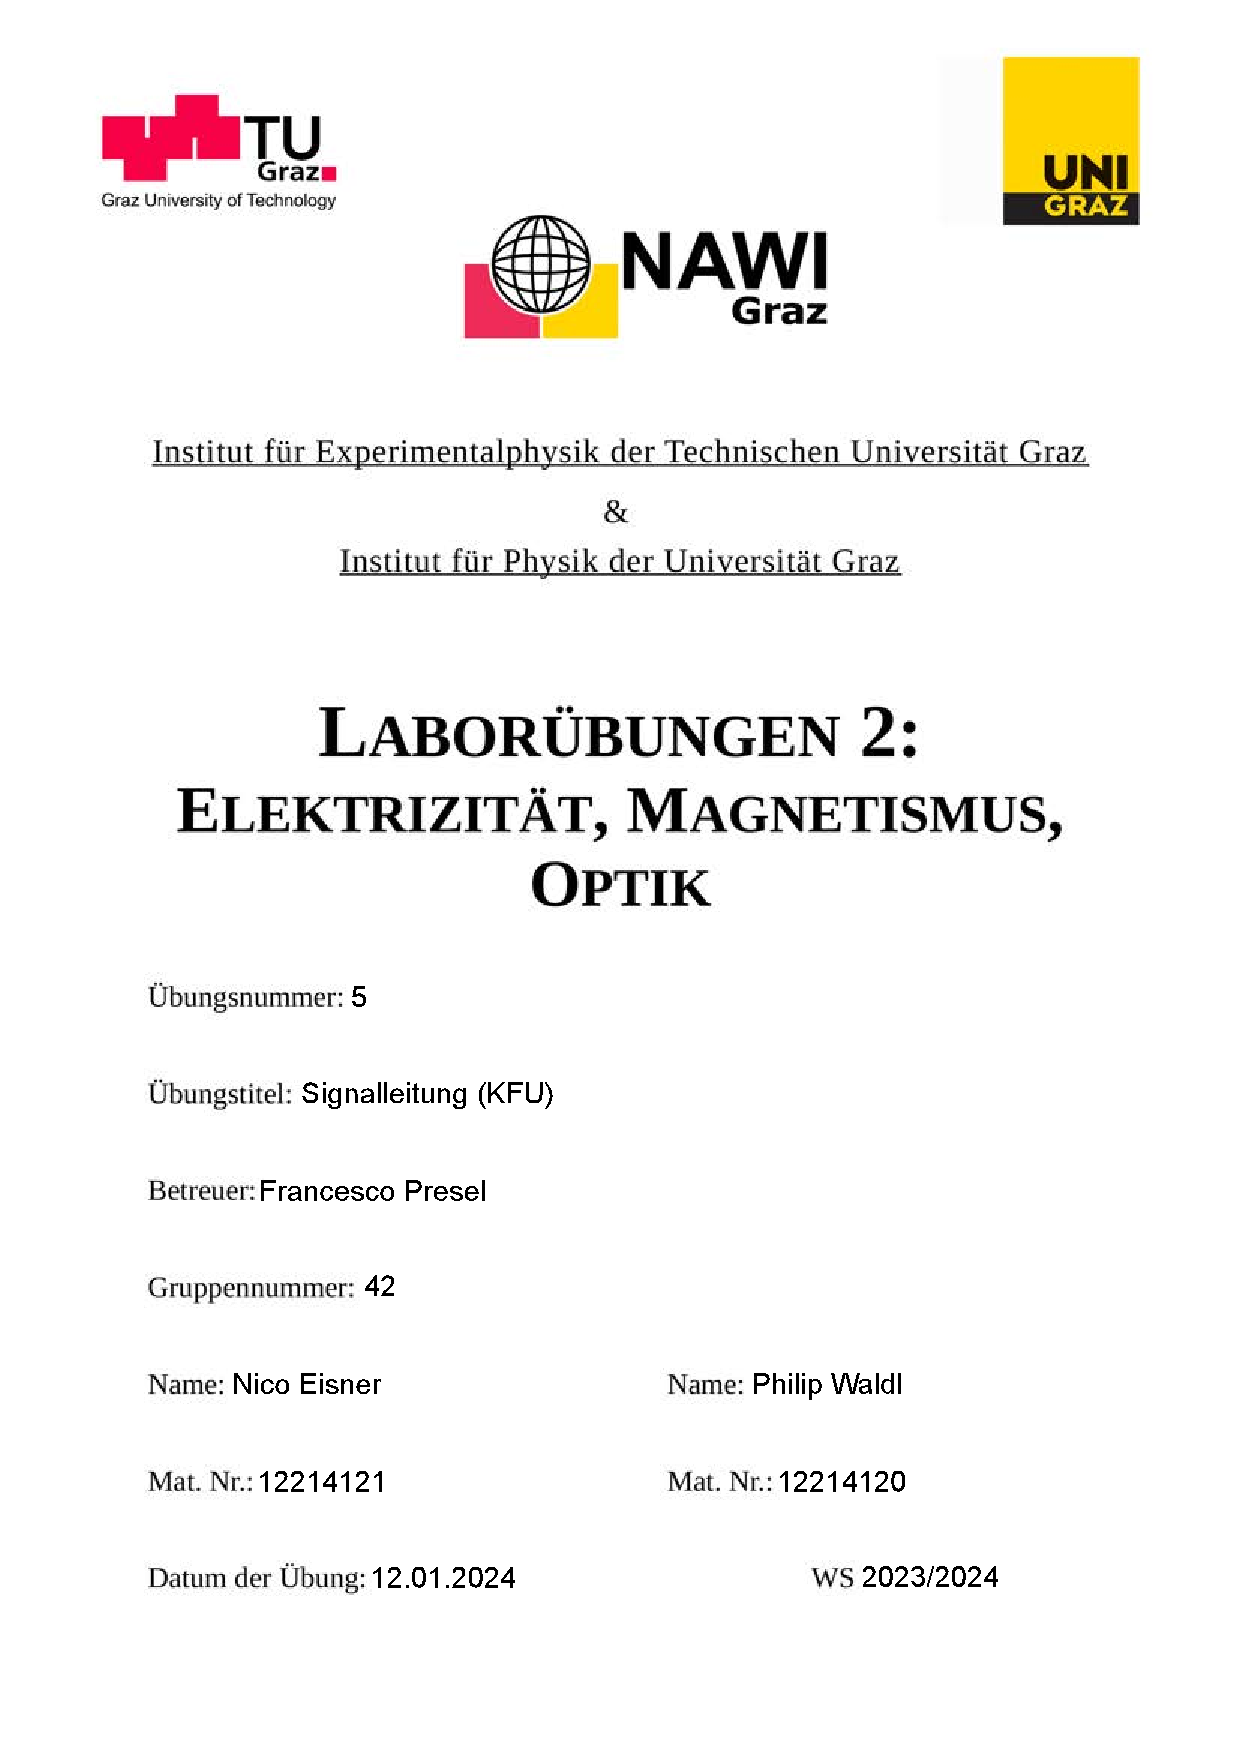
\includepdf[pages={1}]{../Deckblätter/Deckblatt_Signalleitung.pdf}

\tableofcontents
\newpage

\section{Aufgabenstellung} %jo beschreibn wos gmocht host ------------------------------
Der Versuch Signalleitung behandelt, wie der Titel bereits vermuten lässt, das Thema Signalleitung. Dabei wird vor allem Wert auf das Signal bei verschiedenen Widerständen gelegt. 
Weiters sollen aber auch Größen wie Reflexionskoeffizient und Signalgeschwindigkeit bestimmt werden. \newline

\noindent
Die genaue Aufgabenstellung sieht wie folgt aus: 

\begin{itemize}
    \item Messung und Erklärung des zeitlichen Spannungsverlaufes 25-30 m Koaxialkabel bei
    \begin{itemize}
        \item angepasstem Innenwiderstand der Signalquelle
        \item einer Signalquelle mit hohem Innenwiderstand
        \item einer Signalquelle mit niedrigem Innenwiderstand
    \end{itemize}
    \item Bestimmung Reflexionskoeffizient des Kabelendes und Bestimmung der Kabelimpedanz
    \item Bestimmung Signalgeschwindigkeit im Koaxialkabel und relative Permittivität des Isolatormaterials des Koaxialkabels
    \item Dimensionierung der Widerstände für einen passiven, symmetrischen Verzweiger mit Demonstation
\end{itemize}

\noindent
Alle Informationen und Methodiken wurden uns von der Technischen Universität bereitgestellt \cite{teachcenter2}. 



\section{Voraussetzungen \& Grundlagen} %Grundlagen erklären, Formeln mit erklärung


\subsection{Signalausbreitung in Kabeln}

Wenn eine ebene Welle auf ein verschieden dichtes Medium trifft, wird sie teilweiße reflektiert.
Selbiges gilt auch für elektrische Wellen, welche durch einen Leiter laufen und dann auf einen Widerstand treffen. 
Durchläuft ein Spannungspuls also eine Leitung mit offenem Ende, so wird diese dort beim Auftreffen reflektiert und wird in die entgegengesetzte Leitungsrichtung zurückgestoßen.
Bei einem Kabelende mit höherem Widerstand wird das Signal zwar auch reflektiert, jedoch nun gespiegelt.
Dieses Verhalten wird als Reflexionskoeffizient $\rho$ festgehalten und gibt das Verhältnis von reflektiertem- und eingetroffenem Strahl wieder.
Mittels folgender Formel kann dieser Reflexionskoeffizient auch berechnet werden:

\begin{equation}
    \label{eq:Reflexionskoeffizient}
    \centerline{Reflexionskoeffizient \\ $\rho = \frac{U_R}{U_E} = \frac{Z_A - Z_K}{Z_A + Z_K}$ \\ $\Delta \rho = \vert \frac{\partial \rho}{\partial U_R} * \Delta U_R \vert + \vert \frac{\partial \rho}{\partial U_E} * \Delta U_E \vert$}
\end{equation}

\noindent
Deswegen muss bei höherfrequenten Signalen die Leistungs- und Abschlussimpedanz immer aufeinander abgestimmt werden, damit es nicht zu ungewollten Signalüberlagerungen kommen kann.
Bei BNC-Kabeln und BNC-Abschlüssen bzw BNC-Geräten ist dieser Innenwiderstand / Impedanzwert auf 50 $\Omega$ genormt. \newline

\noindent
Außerdem kann für verschiedene Kabel die Signalgeschwindigkeit v je nach Dichte des Leiters bestimmt werden.
Im Optimalfall wäre diese Geschwindigkeit natürlich die Lichtgeschwindigkeit, welche aber in Realität aufgrund der Permittivität des Dielektrikums nicht erreicht wird.

\begin{equation}
    \label{eq:Signalgeschwindigkeit}
    \centerline{Signalgeschwindigkeit \\ $v = \frac{c}{\sqrt{\epsilon_r \mu_r}} = \frac{s}{t}$ \\ $\Delta v = \vert \frac{\partial v}{\partial s} * \Delta s \vert + \vert \frac{\partial v}{\partial t} * \Delta t \vert $}
\end{equation}

\noindent
Dabei gilt 1/$\sqrt{\epsilon_r \mu_r}$ als sogenannter Verkürzungsfaktor, welcher die Signalgeschwindigkeit der Lichtgeschwindigkeit gegenüberstellt.
Der Verkürzungsfaktor von gewöhnlichen Koaxialkabeln liegt dabei bei etwa 66$\%$.

\subsection{Begriffe}

Für diesen Versuch ist es weiters wichtig, einige Begriffe zu kennen und zu verstehen.

\begin{table}[H]
    \centering
    \caption{Definitionen \cite{teachcenter2}}
    \label{tab:definitionen}
    \resizebox{\columnwidth}{!}{\begin{tabular}{|l|l|}
        \hline
        Kapazität & Maß für die Fähigkeit eines Körpers oder Systems, elektrische Ladung zu speichern \cite{Kapazität} \\
        Induktivitätsbelag & Induktivität einer elektrischen Leitung pro Länge dieser Leitung \cite{Leitungsbeläge} \\
        Widerstandsbelag & Widerstand einer elektrischen Leitung pro Länge dieser Leitung \cite{Leitungsbeläge}\\
        Kabelimpedanz & Das Verhältnis von reflektierter und transmittierter Amplitude der Welle an einer Grenzfläche. \cite{Wellenwiderstand} \\
        Abschlussimpedanz & Technische Ausführung eines hochfrequenz-tauglichen Widerstands , der z.B. für Messzwecke \\
         & oder zur Vermeidung von Reflexionen als Last an eine Signalquelle oder Leitung angeschlossen wird. \cite{Abschlusswiderstand} \\
        \hline
    \end{tabular}}
\end{table}


\subsection{Wichtige Zusammenhänge}

\begin{equation}
    \label{eq:Permittivität}
    \centerline{Permittivität \\ $\epsilon_r = \frac{c^2}{v^2} = \frac{s}{t}$ \\ $\Delta \epsilon_r = \vert \frac{\partial \epsilon_r}{\partial v} * \Delta v \vert $}
\end{equation}
    

\section{Versuchsanordnung} %mit skizze kurz beschreiben ------------------------------

Anhand der folgenden Schaltpläne wurden die Schaltungen jeder Aufgabe in die Tat umgesetzt.

\subsection{Spannungsverläufe}

\begin{figure}[H]
    \centering
    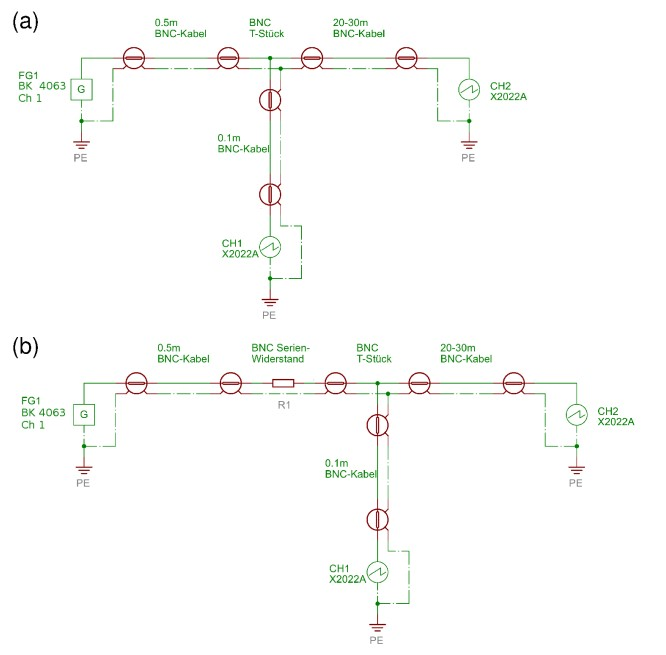
\includegraphics[width=0.4\linewidth]{nudes/Aufgabe 1 Schaltplan.jpg}
    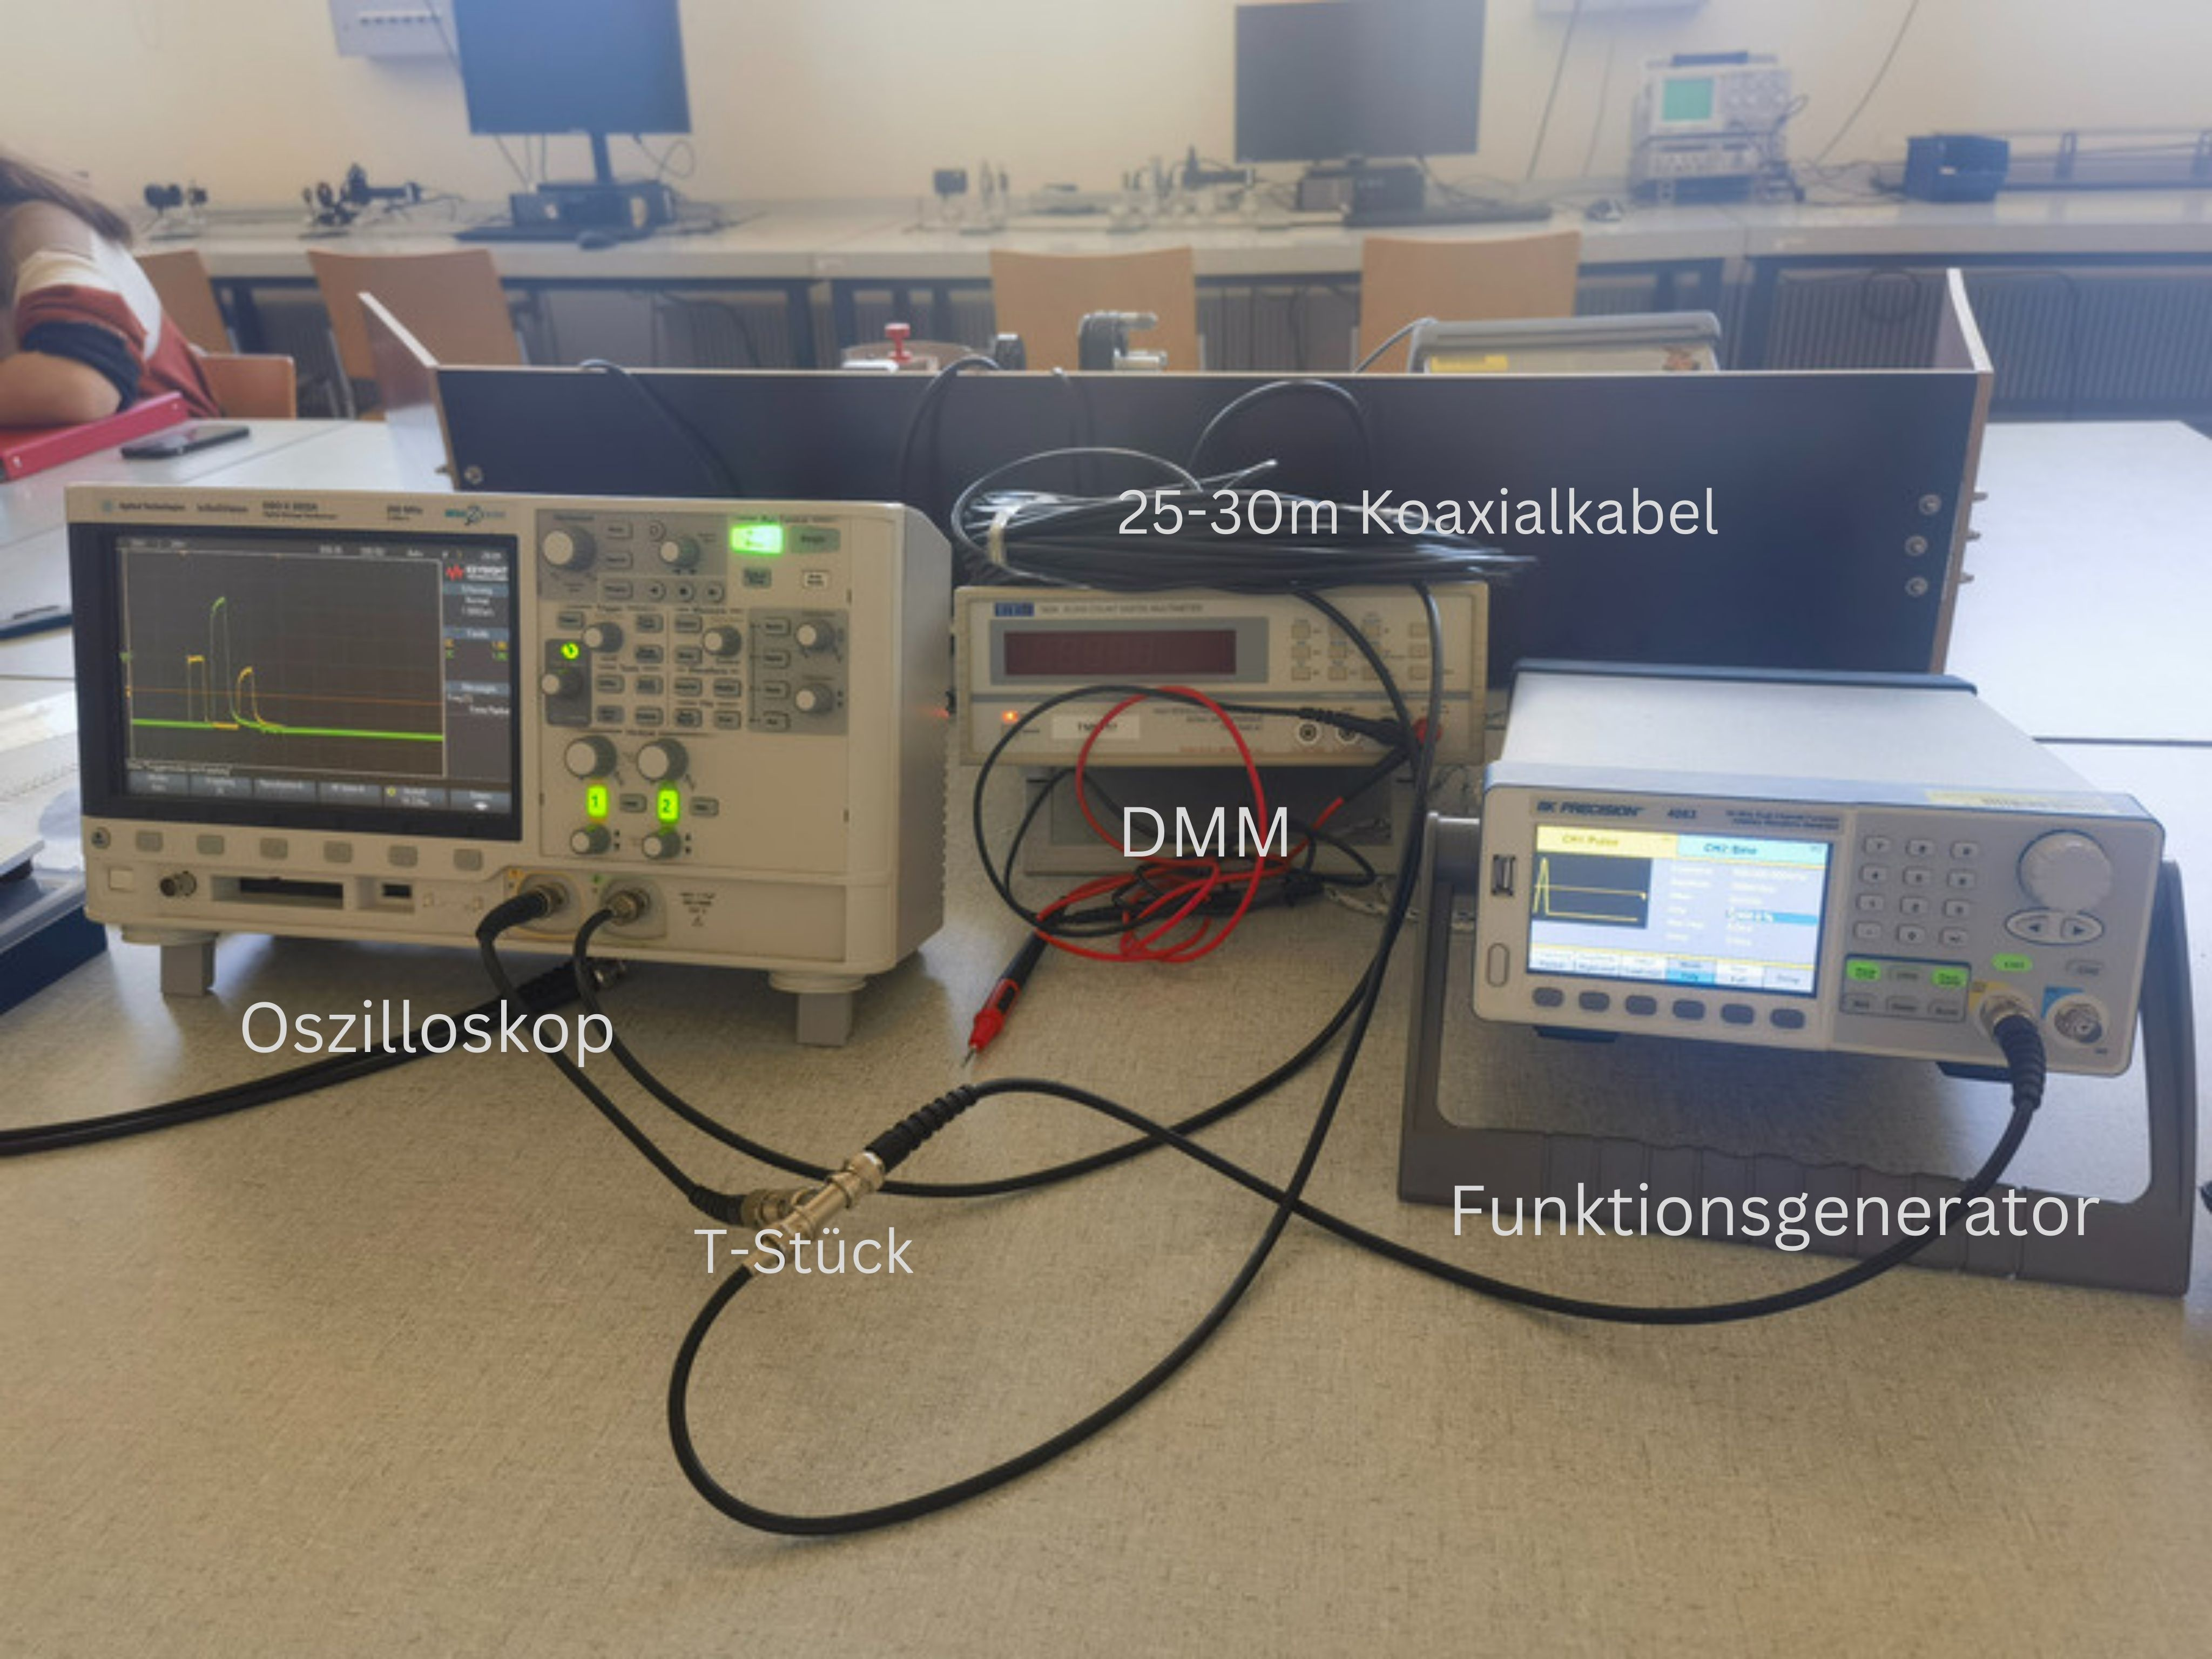
\includegraphics[width=0.4\linewidth]{nudes/Aufbau1.jpg}
    \caption{Schaltplan und realer Aufbau der ersten Aufgabe}
    \label{fig:Aufbau1}
\end{figure}

\subsection{Reflexionskoeffizient/Kabelimpedanz}

\begin{figure}[H]
    \centering
    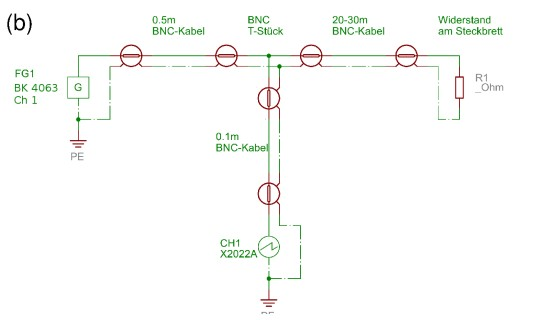
\includegraphics[width=0.4\linewidth]{nudes/Aufgabe 2,3 Schaltplan.jpg}
    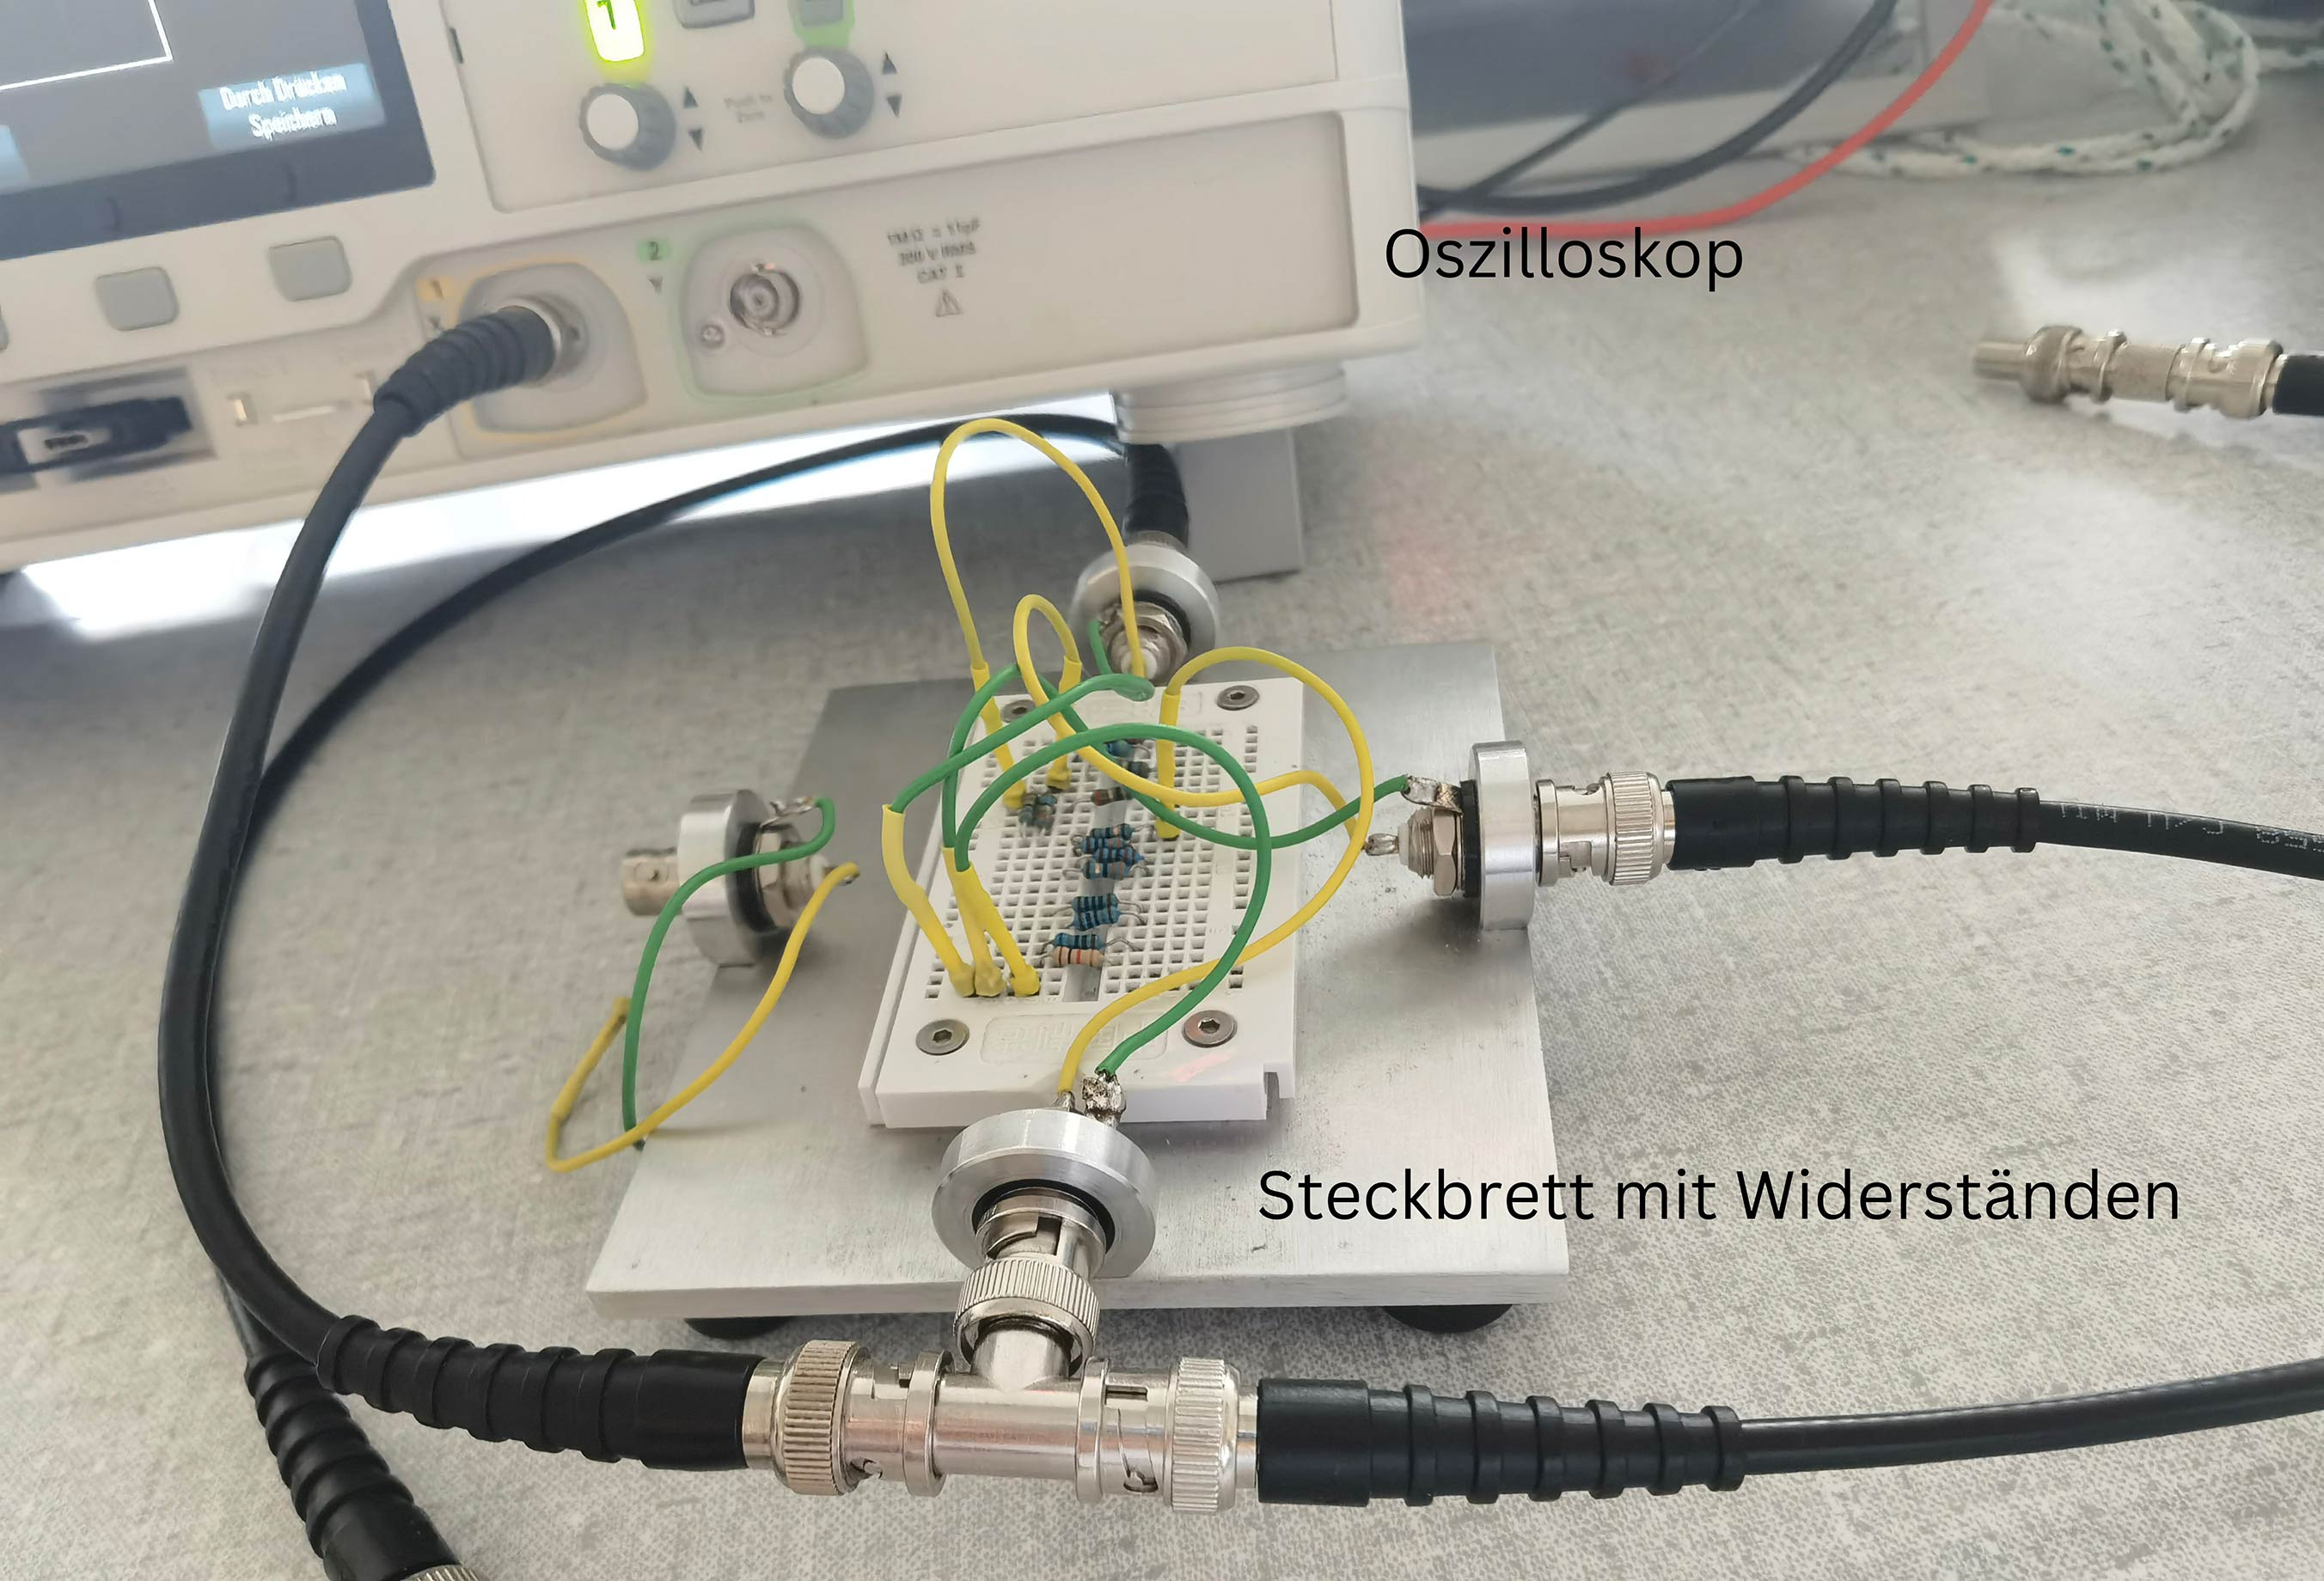
\includegraphics[width=0.4\linewidth]{nudes/Aufbau2.jpg}
    \caption{Schaltplan und realer Aufbau der zweiten Aufgabe}
    \label{fig:Aufbau2}
\end{figure}

\subsection{Signalgeschwindigkeit/relative Permittivität}

\begin{figure}[H]
    \centering
    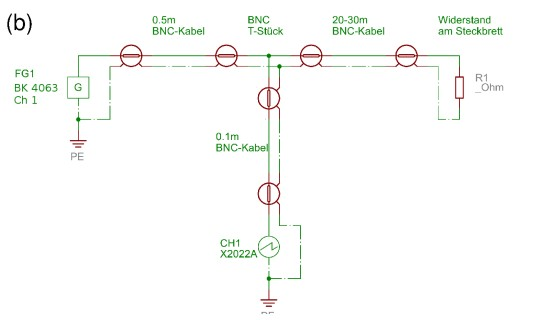
\includegraphics[width=0.4\linewidth]{nudes/Aufgabe 2,3 Schaltplan.jpg}
    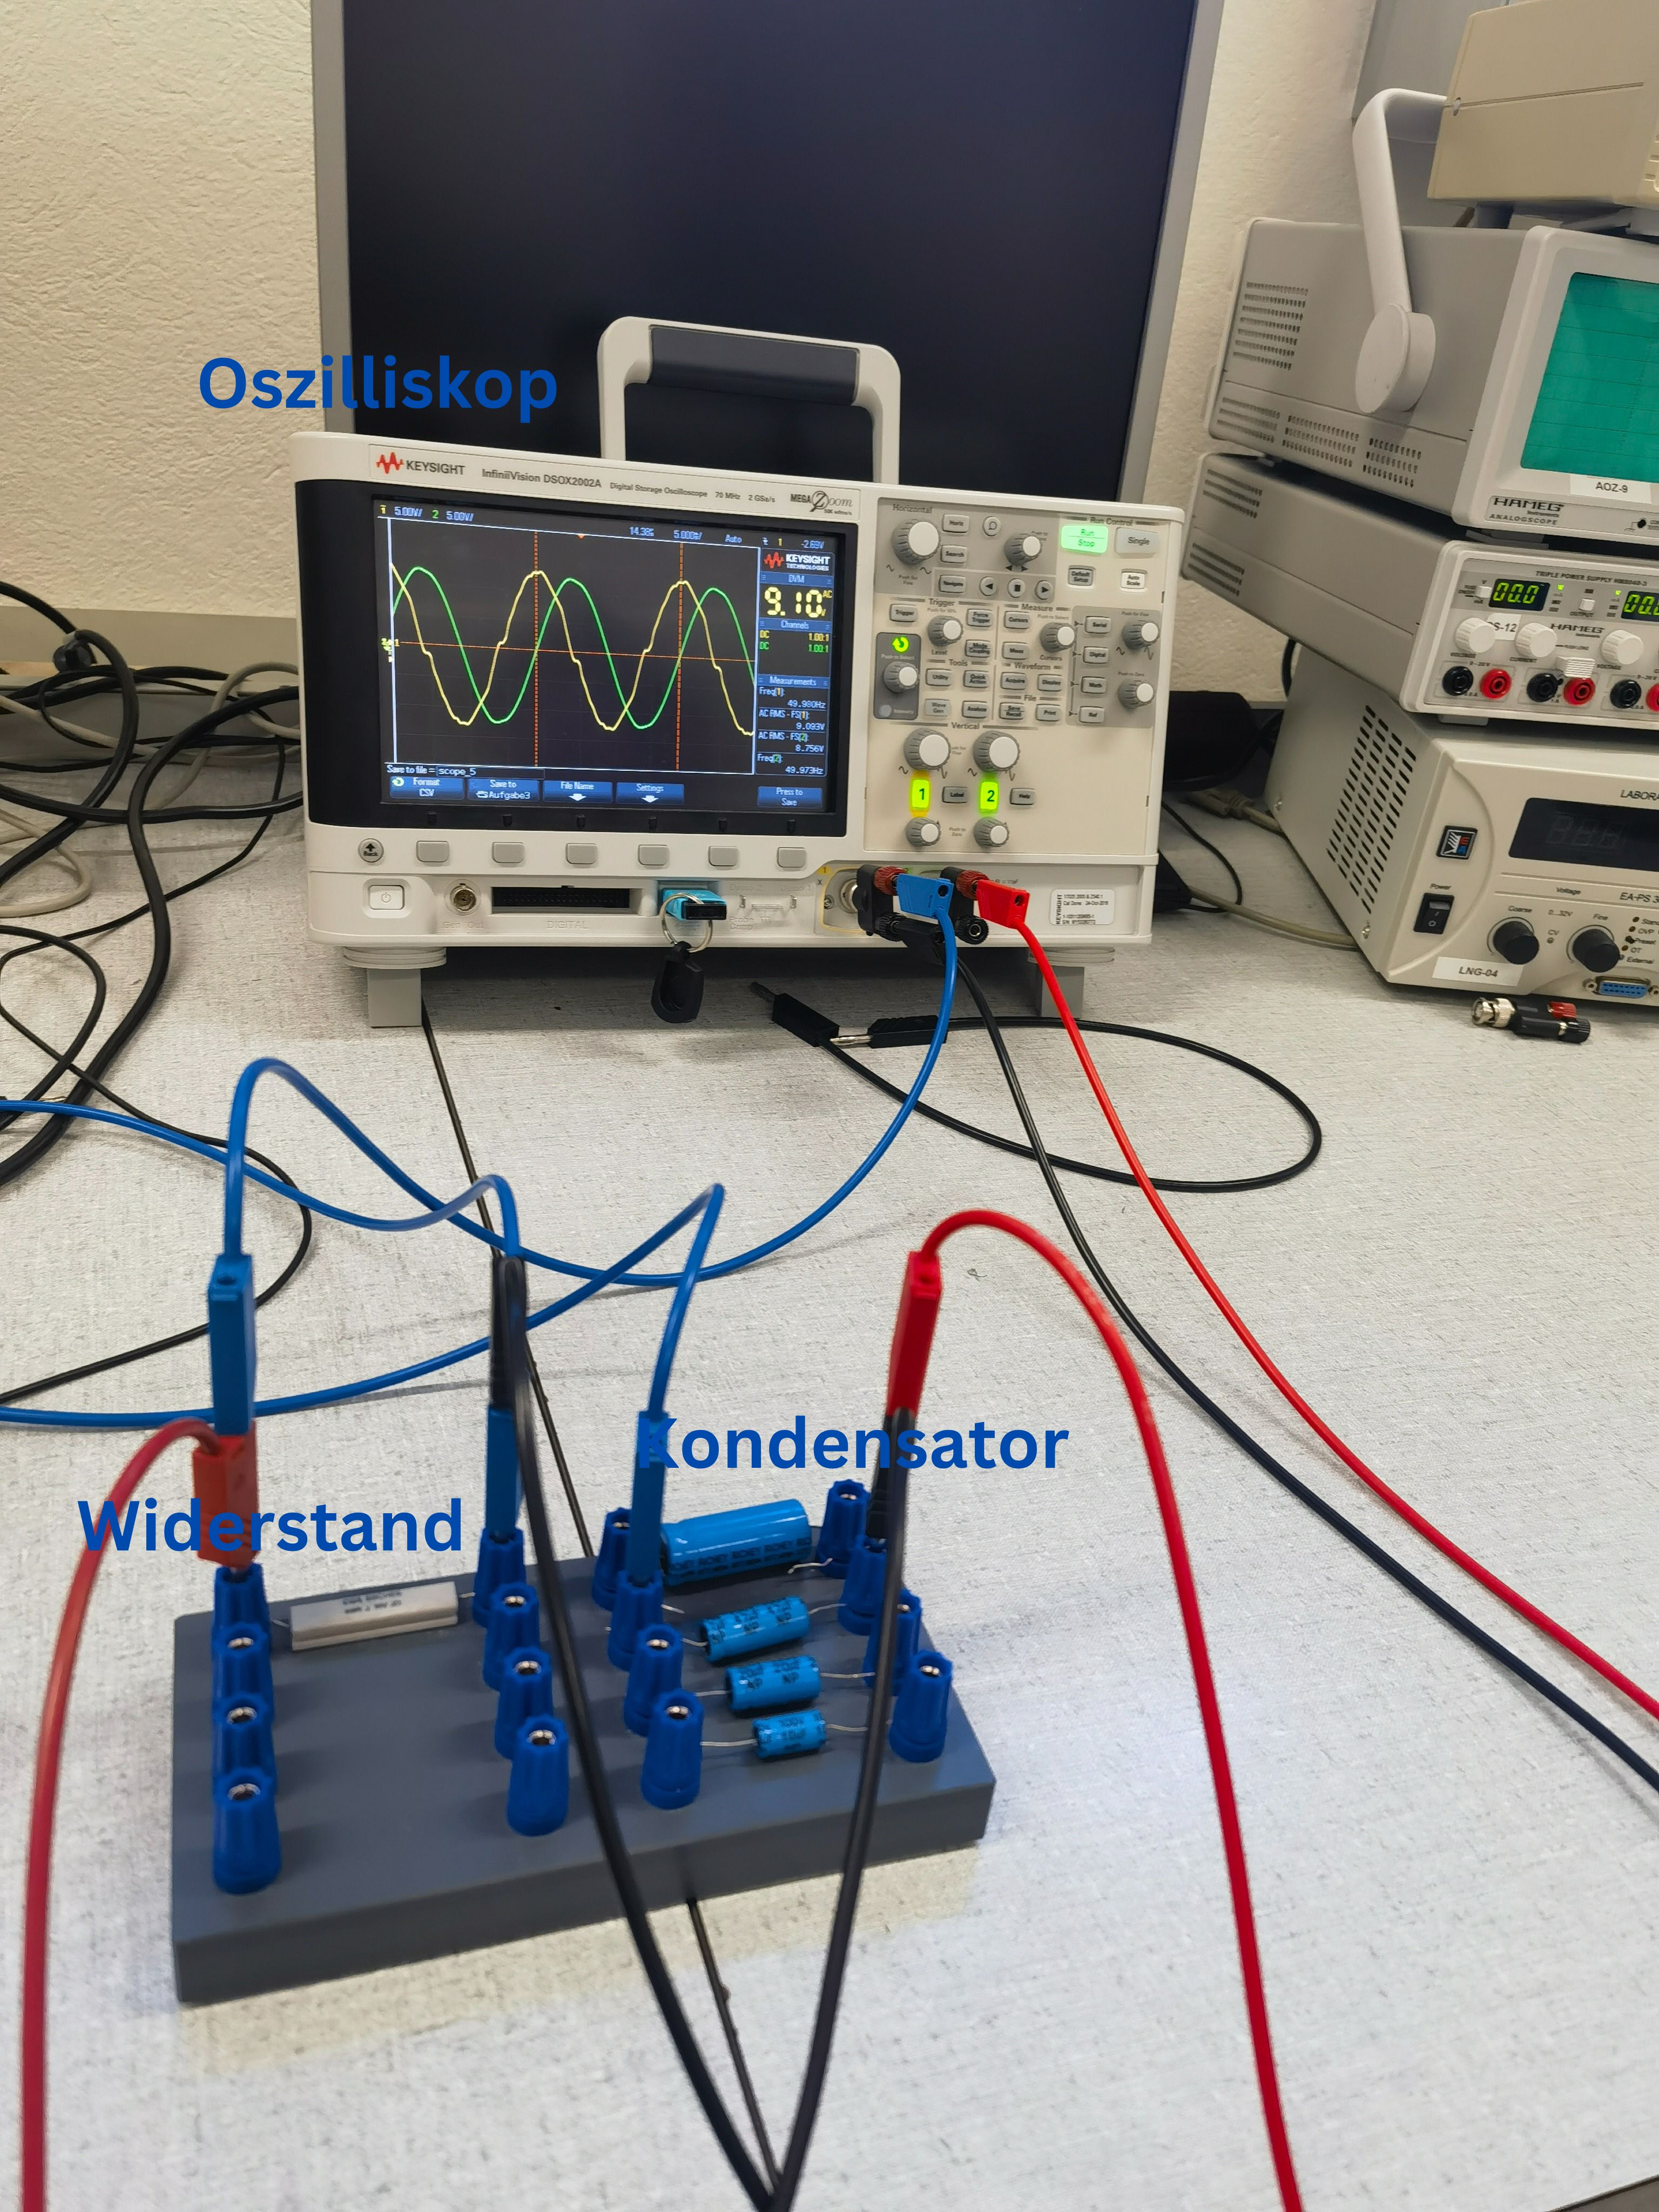
\includegraphics[width=0.4\linewidth, angle=90]{nudes/Aufbau3.jpg}
    \caption{Schaltplan und Steckbrett mit verschiedenen Abschlusswiderständen}
    \label{fig:Aufbau3}
\end{figure}

\subsection{Verzweiger}

\begin{figure}[H]
    \centering
    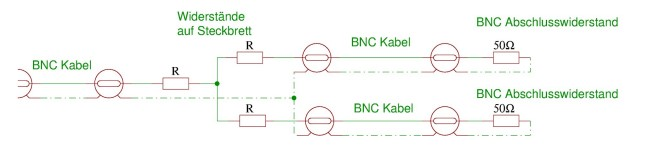
\includegraphics[width=0.4\linewidth]{nudes/Aufgabe 4 Schaltplan.jpg}
    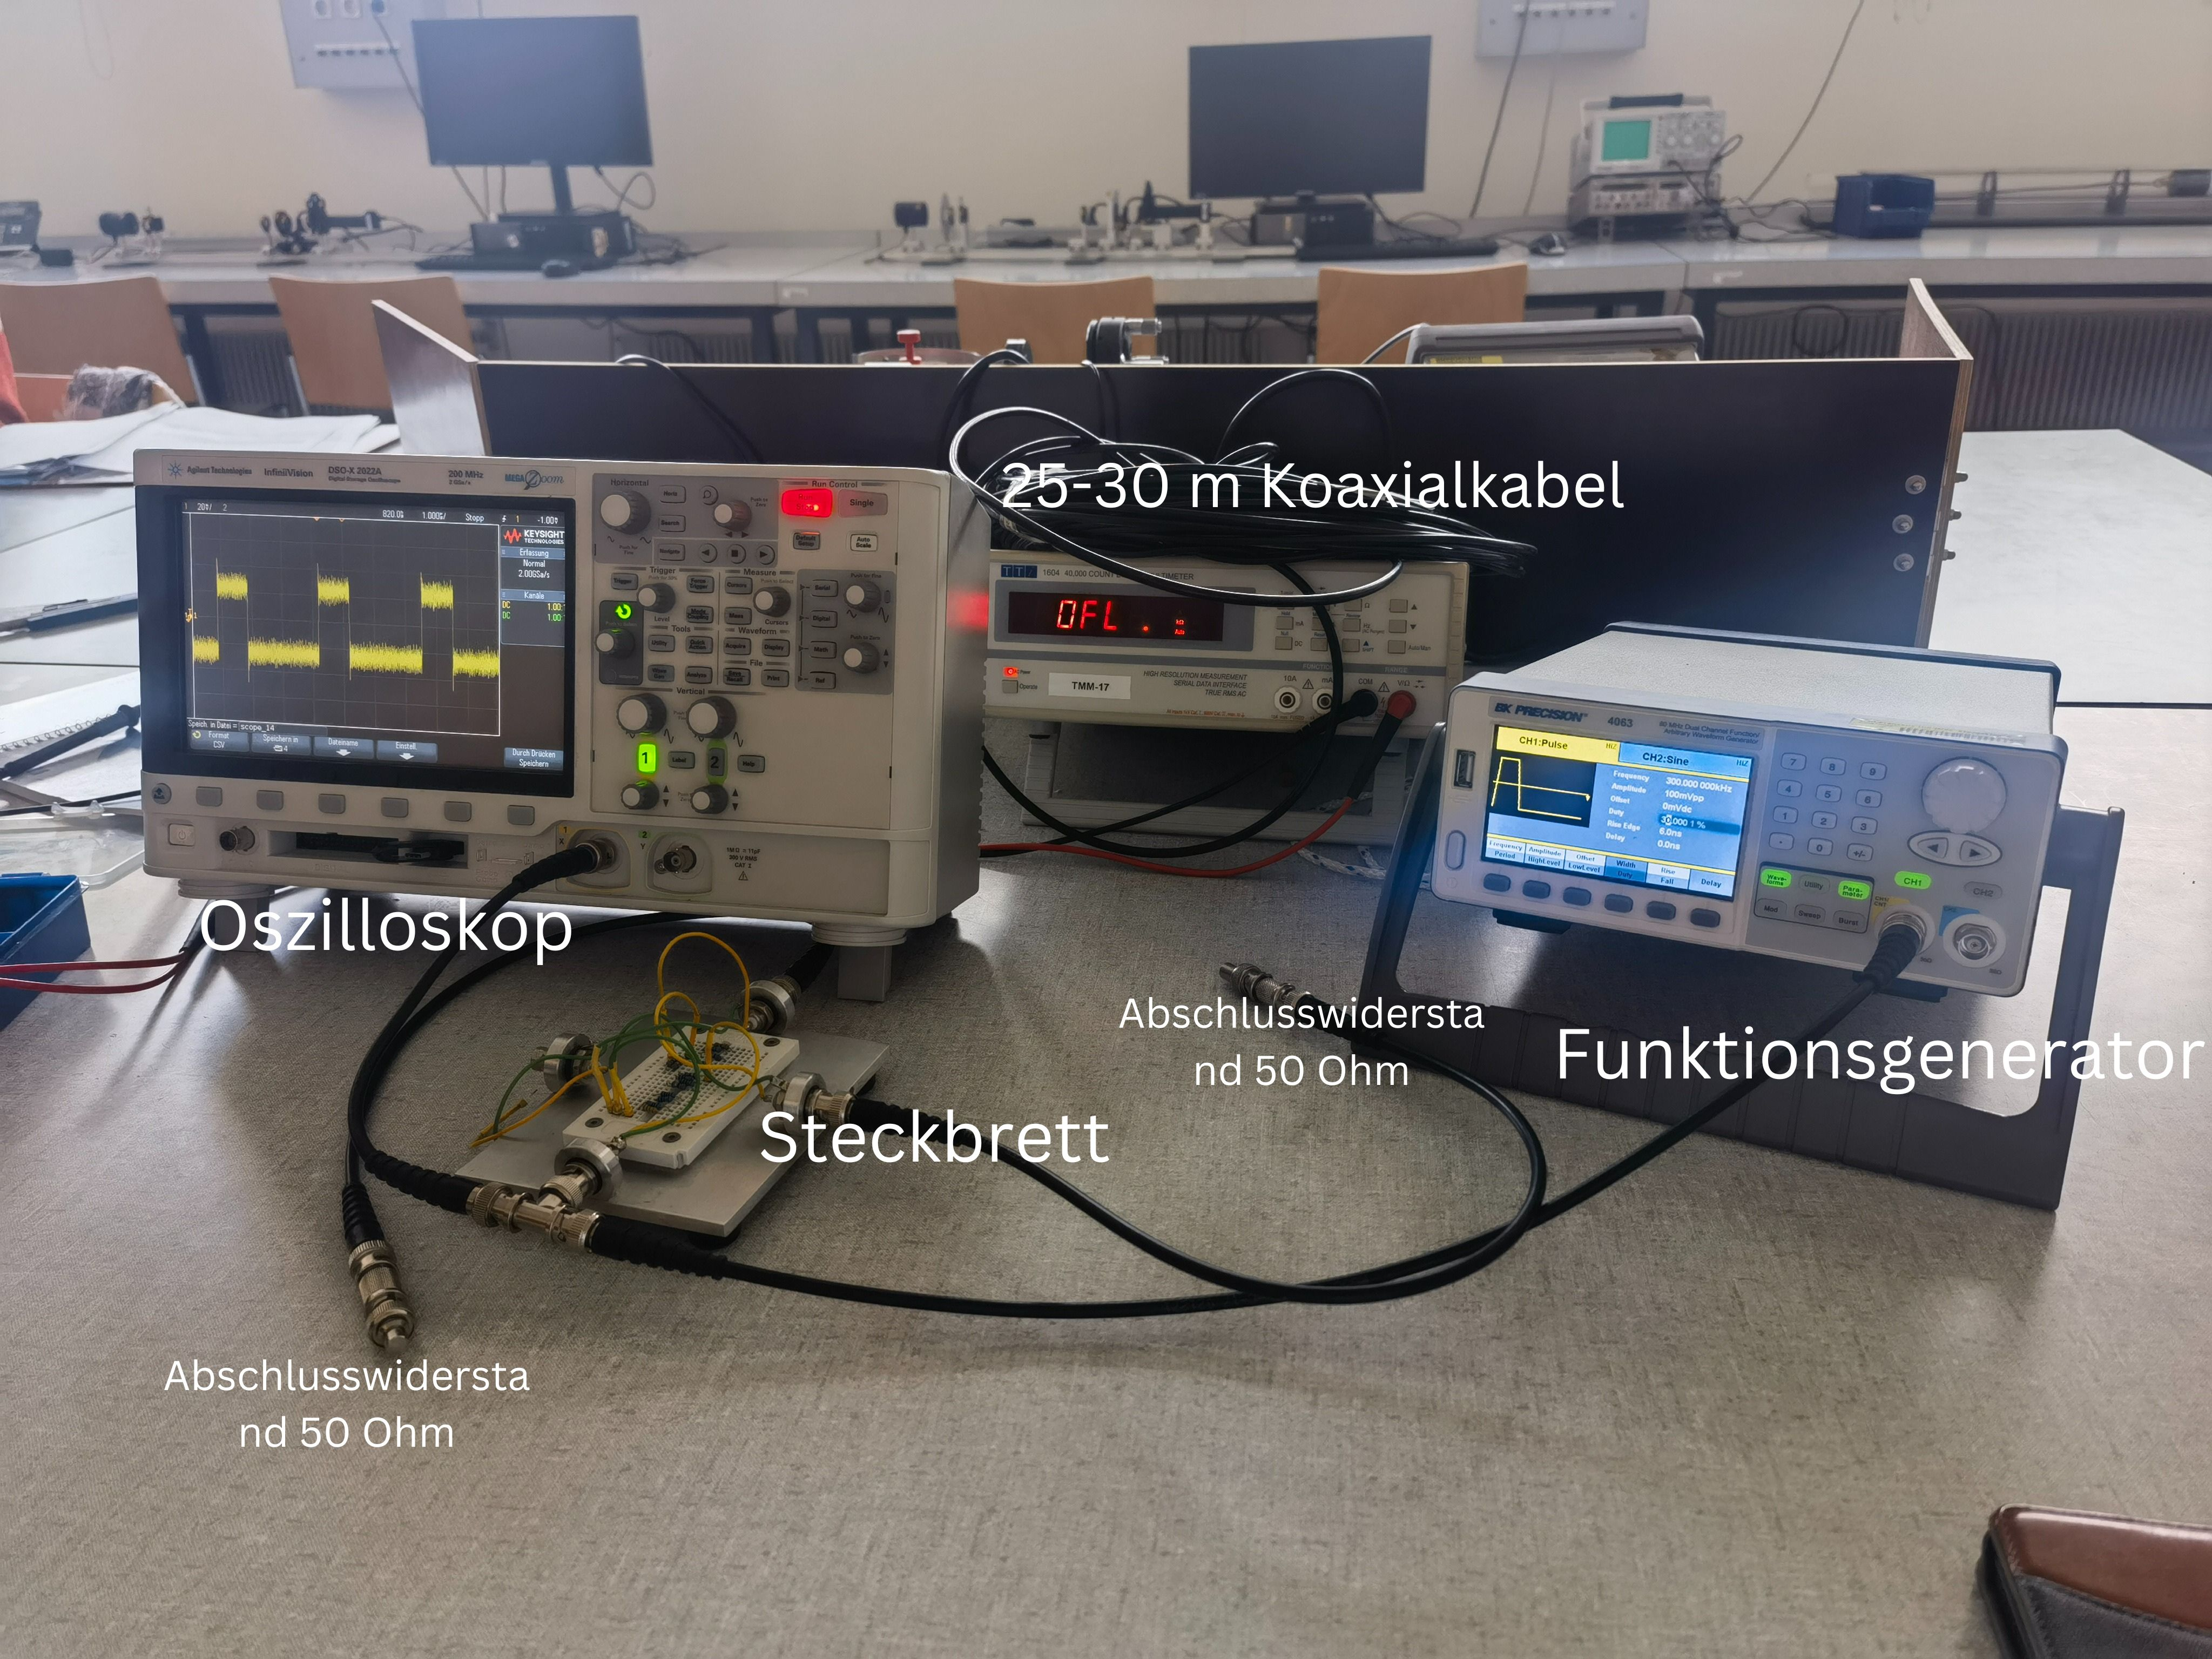
\includegraphics[width=0.4\linewidth]{nudes/Aufbau4.jpg}
    \caption{Schaltplan und realer Aufbau der vierten Aufgabe}
    \label{fig:Aufbau4}
\end{figure}


    
\section{Geräteliste} %jo holt a listn ------------------------------

\begin{table}[H]
    \centering
    \caption{Im Versuch verwendete Geräte und Utensilien.}
    \label{tab:geraete}
    \begin{tabular}{| l | l | l |}
        \hline
        Gerät   & Gerätenummer  & Unsicherheit \\
        \hline
        Oszilloskop & {n.a} & 30 mV \\
        Digitalmultimeter & TTi 1604 & 1.5 $\%$ ± 6 dig \\
        Funktionsgenerator & {n.a} & {n.a} \\
        Widerstände & {n.a} & {n.a} \\
        BNC-Kabel & {n.a} & {n.a} \\
        Abschlusswiderstände & {n.a} & {n.a} \\
        Steckbrett & {n.a} & {n.a} \\
        \hline
    \end{tabular}
\end{table}


\section{Versuchsdurchführung \& Messergebnisse} %nachvollziehbar und klar dargestellt ------------------------------

\subsection{Spannungsverläufe}

Bei der ersten Aufgabe wurde zunächst die Schaltung laut \ref{fig:Aufbau1} umgesetzt. 
Am Frequenzgenerator wird dann ein rechteckiges Pulssignal mit 300 kHz und einer Pulsdauer von 100 nS (3$\$$ Duty) eingestellt.
Dieses Signal wird dann über die Schaltung am Oszilloskop dargestellt. 
Dann wird die Pulsdauer schrittweiße bis auf 30$\%$ Duty erhöht und die resultierenden Oszigraphen als Bilder gespeichert.

\begin{figure}[H]
    \centering
    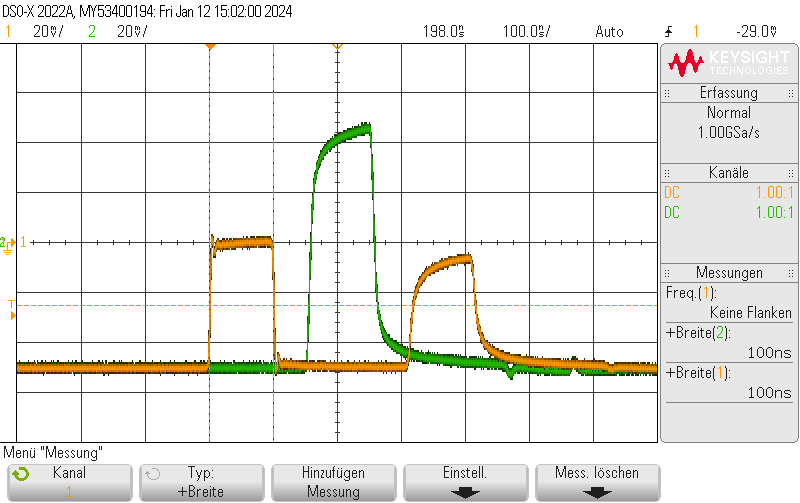
\includegraphics[width=0.4\linewidth]{nudes/Messungen/1/a/scope_1.png}
    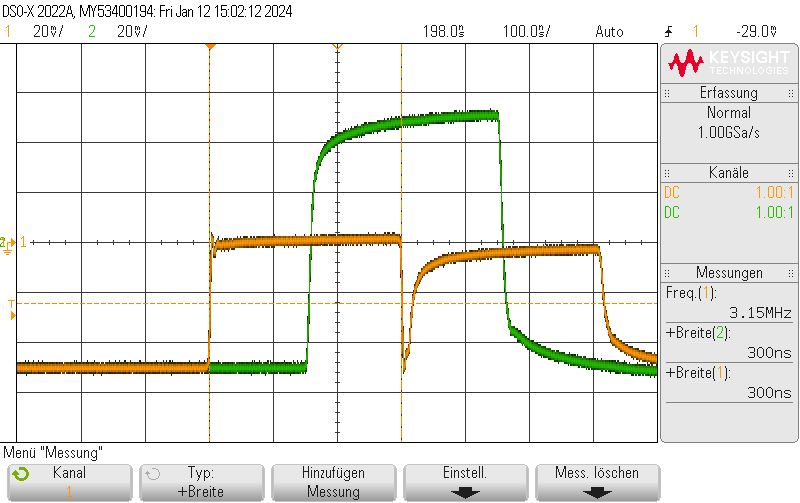
\includegraphics[width=0.4\linewidth]{nudes/Messungen/1/a/scope_2.png}
    \caption{Resultierende Graphen bei Pulsdauer 100 nS und 300 nS}
    \label{fig:GraphenA1}
\end{figure}

\begin{figure}[H]
    \centering
    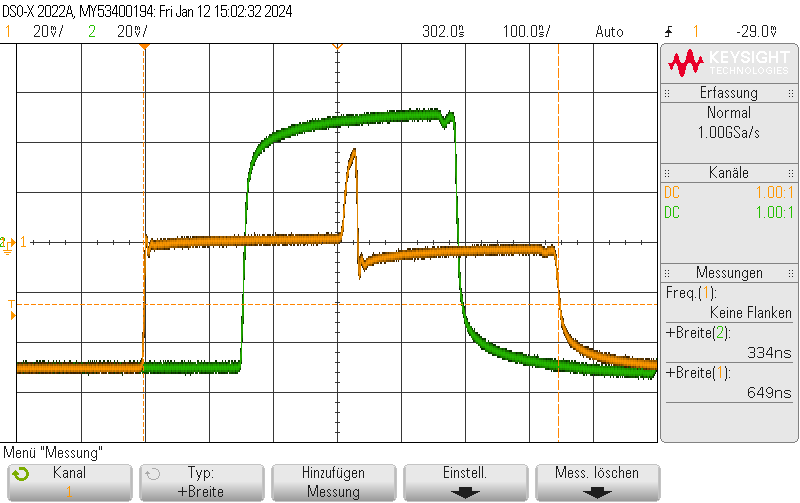
\includegraphics[width=0.4\linewidth]{nudes/Messungen/1/a/scope_3.png}
    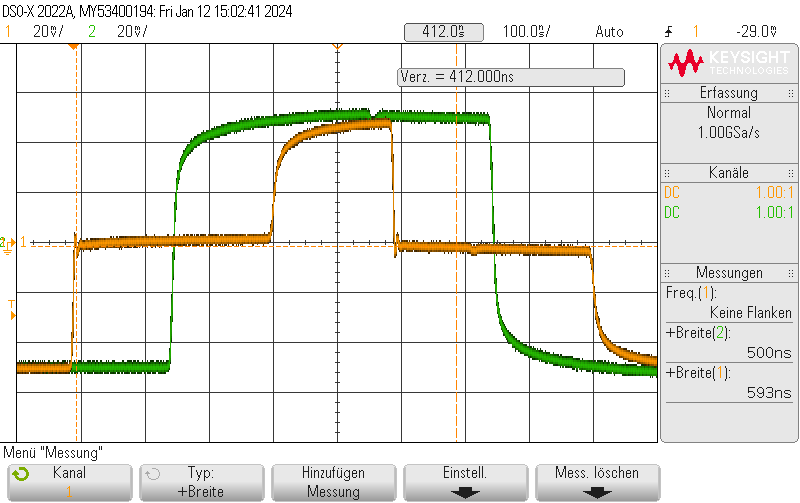
\includegraphics[width=0.4\linewidth]{nudes/Messungen/1/a/scope_4.png}
    \caption{Resultierende Graphen bei Pulsdauer 335 nS und 500 nS}
    \label{fig:GraphenA2}
\end{figure}

\begin{figure}[H]
    \centering
    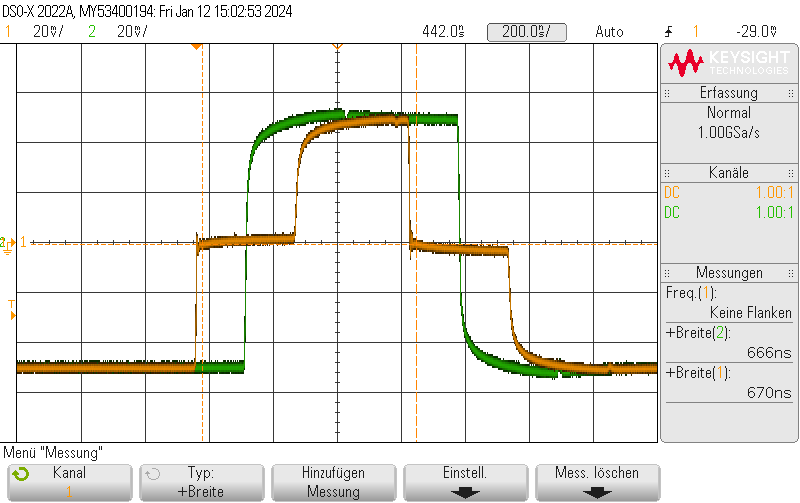
\includegraphics[width=0.4\linewidth]{nudes/Messungen/1/a/scope_5.png}
    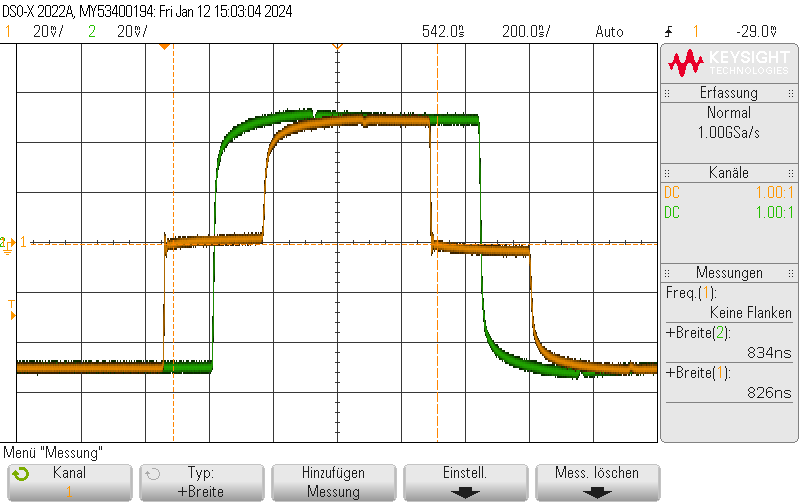
\includegraphics[width=0.4\linewidth]{nudes/Messungen/1/a/scope_6.png}
    \caption{Resultierende Graphen bei Pulsdauer 666 nS und 834 nS}
    \label{fig:GraphenA3}
\end{figure}

\noindent
Dann wird der Innenwiderstand der Signalquelle durch einen seriell angeschlossenen Widerstand erhöht.
Die Pulsdauer wird auf 1 $\mu S$ eingestellt und das Oszilloskopbild aufgenommen.

\begin{figure}[H]
    \centering
    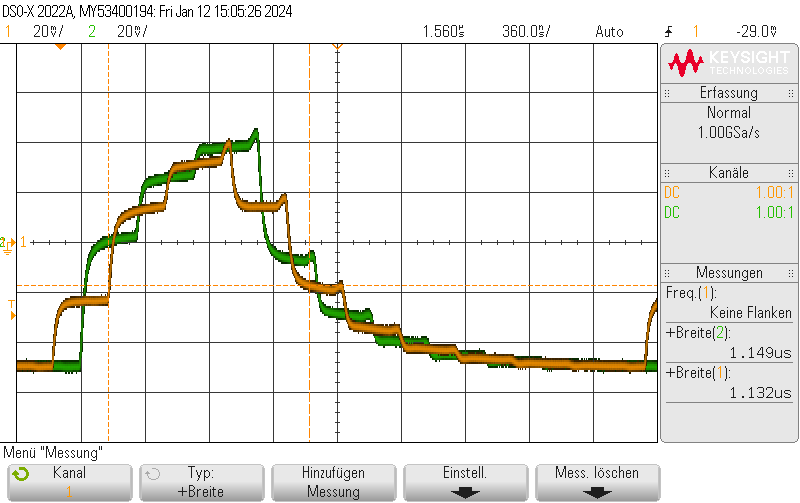
\includegraphics[width=0.6\linewidth]{nudes/Messungen/1/b/scope_8.png}
    \caption{Resultierende Graphen bei erhöhtem Innenwiderstand}
    \label{fig:GraphenB1}
\end{figure}

\noindent
Im Gegensatz dazu wird der Innenwiderstand durch einen paralell geschaltenen Widerstand verringert.
Auch hier wird wieder ein Oszibild gespeichert.

\begin{figure}[H]
    \centering
    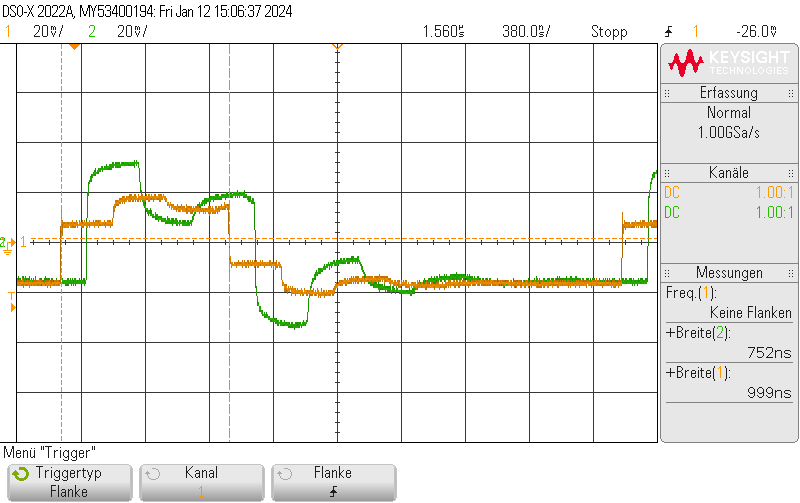
\includegraphics[width=0.6\linewidth]{nudes/Messungen/1/c/scope_9.png}
    \caption{Resultierende Graphen bei verringertem Innenwiderstand}
    \label{fig:GraphenB2}
\end{figure}


\subsection{Reflexionskoeffizient/Kabelimpedanz}

Beim zweiten Teil des Versuches werden die Widerstände des Steckbrettes als Abschlusswiderstände genützt, um weiters mittels umgebauter Schaltung \ref{fig:Aufbau2} die Reflexionskoeffizienten für die jeweiligen Widerstände zu bestimmen.
Zunächst wurden jedoch die Widerstände am Steckbrett der Reihe nach mit einem Digitalmultimeter vermessen und die resultierenden Werte festgehalten.

\begin{table}[H]
    \centering
    \caption{Widerstände am Steckbrett}
    \label{tab:Widerstände}
    \begin{tabular}{| l | l |}
        \hline
        R / $\Omega$ & $\Delta R$  \\
        \hline
       0.676 & 0.017 \\
       0.998 & 0.021 \\
         2.2 & 0.1   \\
        16.1 & 0.9   \\
        16.1 & 0.9   \\
        18.2 & 0.9   \\
        22.1 & 1.0   \\
        33.1 & 1.1   \\
        47.2 & 1.4   \\
        68.6 & 1.7   \\
       100.2 & 2.2   \\
         179 & 8     \\
         330 & 11    \\
        \hline
    \end{tabular}
\end{table}

\noindent
Weiters wurden nun die Spannungen $U_E$ und $U_R$ zur späteren Bestimmung der Reflexionskoeffizienten aufgezeichnet.

\begin{table}[H]
    \centering
    \caption{$U_E$ und $U_R$ mit verschiedenen Abschlusswiderständen gemessen}
    \label{tab:A2Spannungen}
    \begin{tabular}{| l | l | l | l |}
        \hline
        R / $\Omega$ & $\Delta R$ & $U_E$ $\pm$ 30 / mV & $U_R$ $\pm$ 30 / mV \\
        \hline
       0.676 & 0.017 & 53 & -42 \\
       0.998 & 0.021 & 54 & -43 \\
         2.2 & 0.1   & 53 & -45 \\
        16.1 & 0.9   & 53 & -28 \\
        16.1 & 0.9   & 53 & -28 \\
        18.2 & 0.9   & 53 & -27 \\
        22.1 & 1.0   & 55 & -21 \\
        33.1 & 1.1   & 53 & -17 \\
        47.2 & 1.4   & 53 &  -7 \\
        68.6 & 1.7   & 53 &   9 \\
       100.2 & 2.2   & 53 &  17 \\
         179 & 8     & 53 &  27 \\
         330 & 11    & 54 &  36 \\
        \hline
    \end{tabular}
\end{table}

\noindent
Nun sollen diese Ergebnisse noch jenen mit einem BNC-Abschlusswiderstandes ermittelt und später verglichen werden.
Dafür wurde dieser in die Schaltung eingebracht und die beiden Werte für $U_E$ und $U_R$ erneut niedergeschrieben.

\begin{table}[H]
    \centering
    \caption{$U_E$ und $U_R$ mit BNC-Abschlusswiderstand gemessen}
    \label{tab:A2SpannungenBNC}
    \begin{tabular}{| l | l |}
        \hline
        $U_E$ $\pm$ 30 / mV & $U_R$ $\pm$ 30 / mV \\
        \hline
        56 & 9 \\
        \hline
    \end{tabular}
\end{table}


\subsection{Signalgeschwindigkeit/relative Permittivität}

Für die Auswertung der dritten Aufgabe wurden keine neuen Daten aufgenommen, da diese mit den Werten aus Aufgabe 1 durchgeführt wird.

\subsection{Verzweiger}

Für den letzten Aufgabenteil wurde die Schaltung gemäß Abbildung \ref{fig:Aufbau4} umgebaut.
Nun gilt es, die richtigen Widerstände am Steckbrett zu finden, damit die Schaltung als Verzweiger funktioniert.
Da sich diese im Bereich der BNC-Elemente (50 $\Omega$) befinden müssten und es von den ca. 16 $\Omega$ Widerständen die benötigten zwei gibt, wurde der gesuchte Bereich hier vermutet.
Dann werden diese Widerstände am Steckbrett ausprobiert und die Oszilloskopbilder paralell dazu beobachtet.
Sobald das reflektierende Signal minimal wird, ist der gesuchte Aufbau gefunden.
Resultierend wurden so die beiden (16.1 $\pm$ 0.9) $\Omega$ Widerstände verwendet, um folgendes Oszi-Resultat zu erhalten.

\begin{figure}[H]
    \centering
    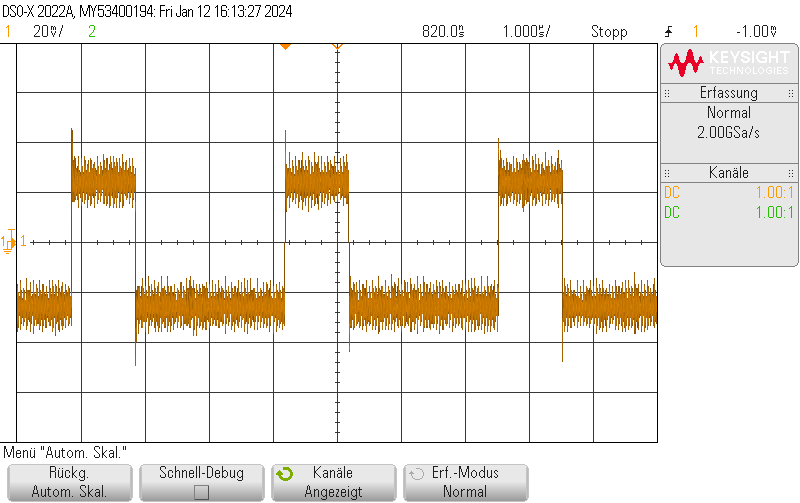
\includegraphics[width=0.6\linewidth]{nudes/Messungen/4/scope_12.png}
    \caption{Resultierende Graphen des Verzweigers}
    \label{fig:GraphA4}
\end{figure}


\section{Auswertung und Unsicherheitsanalyse} %Nicht nur zahlen angeben ------------------------------

In der Auswertung werden zur erhöhten Genauigkeit durchgehend ungerundete Werte bis zu den Endergebnissen verwendet und nur zur Darstellung gerundet. \\
Zur Berechnung der Unsicherheiten wird, wenn nicht anders angegeben, die Größtunsicherheitsmethode verwendet, bei den Graphen werden jedoch für die Unsicherheiten die Standardabweichungen der Mittelwerte herangezogen. 

\subsection{Spannungsverläufe}

Die verschiedenen Spannungsverläufe der jeweiligen Pulsdauern sind in folgender Abbildung zur besseren visualisierung übereinandergestellt.

\begin{figure}[H]
    \centering
    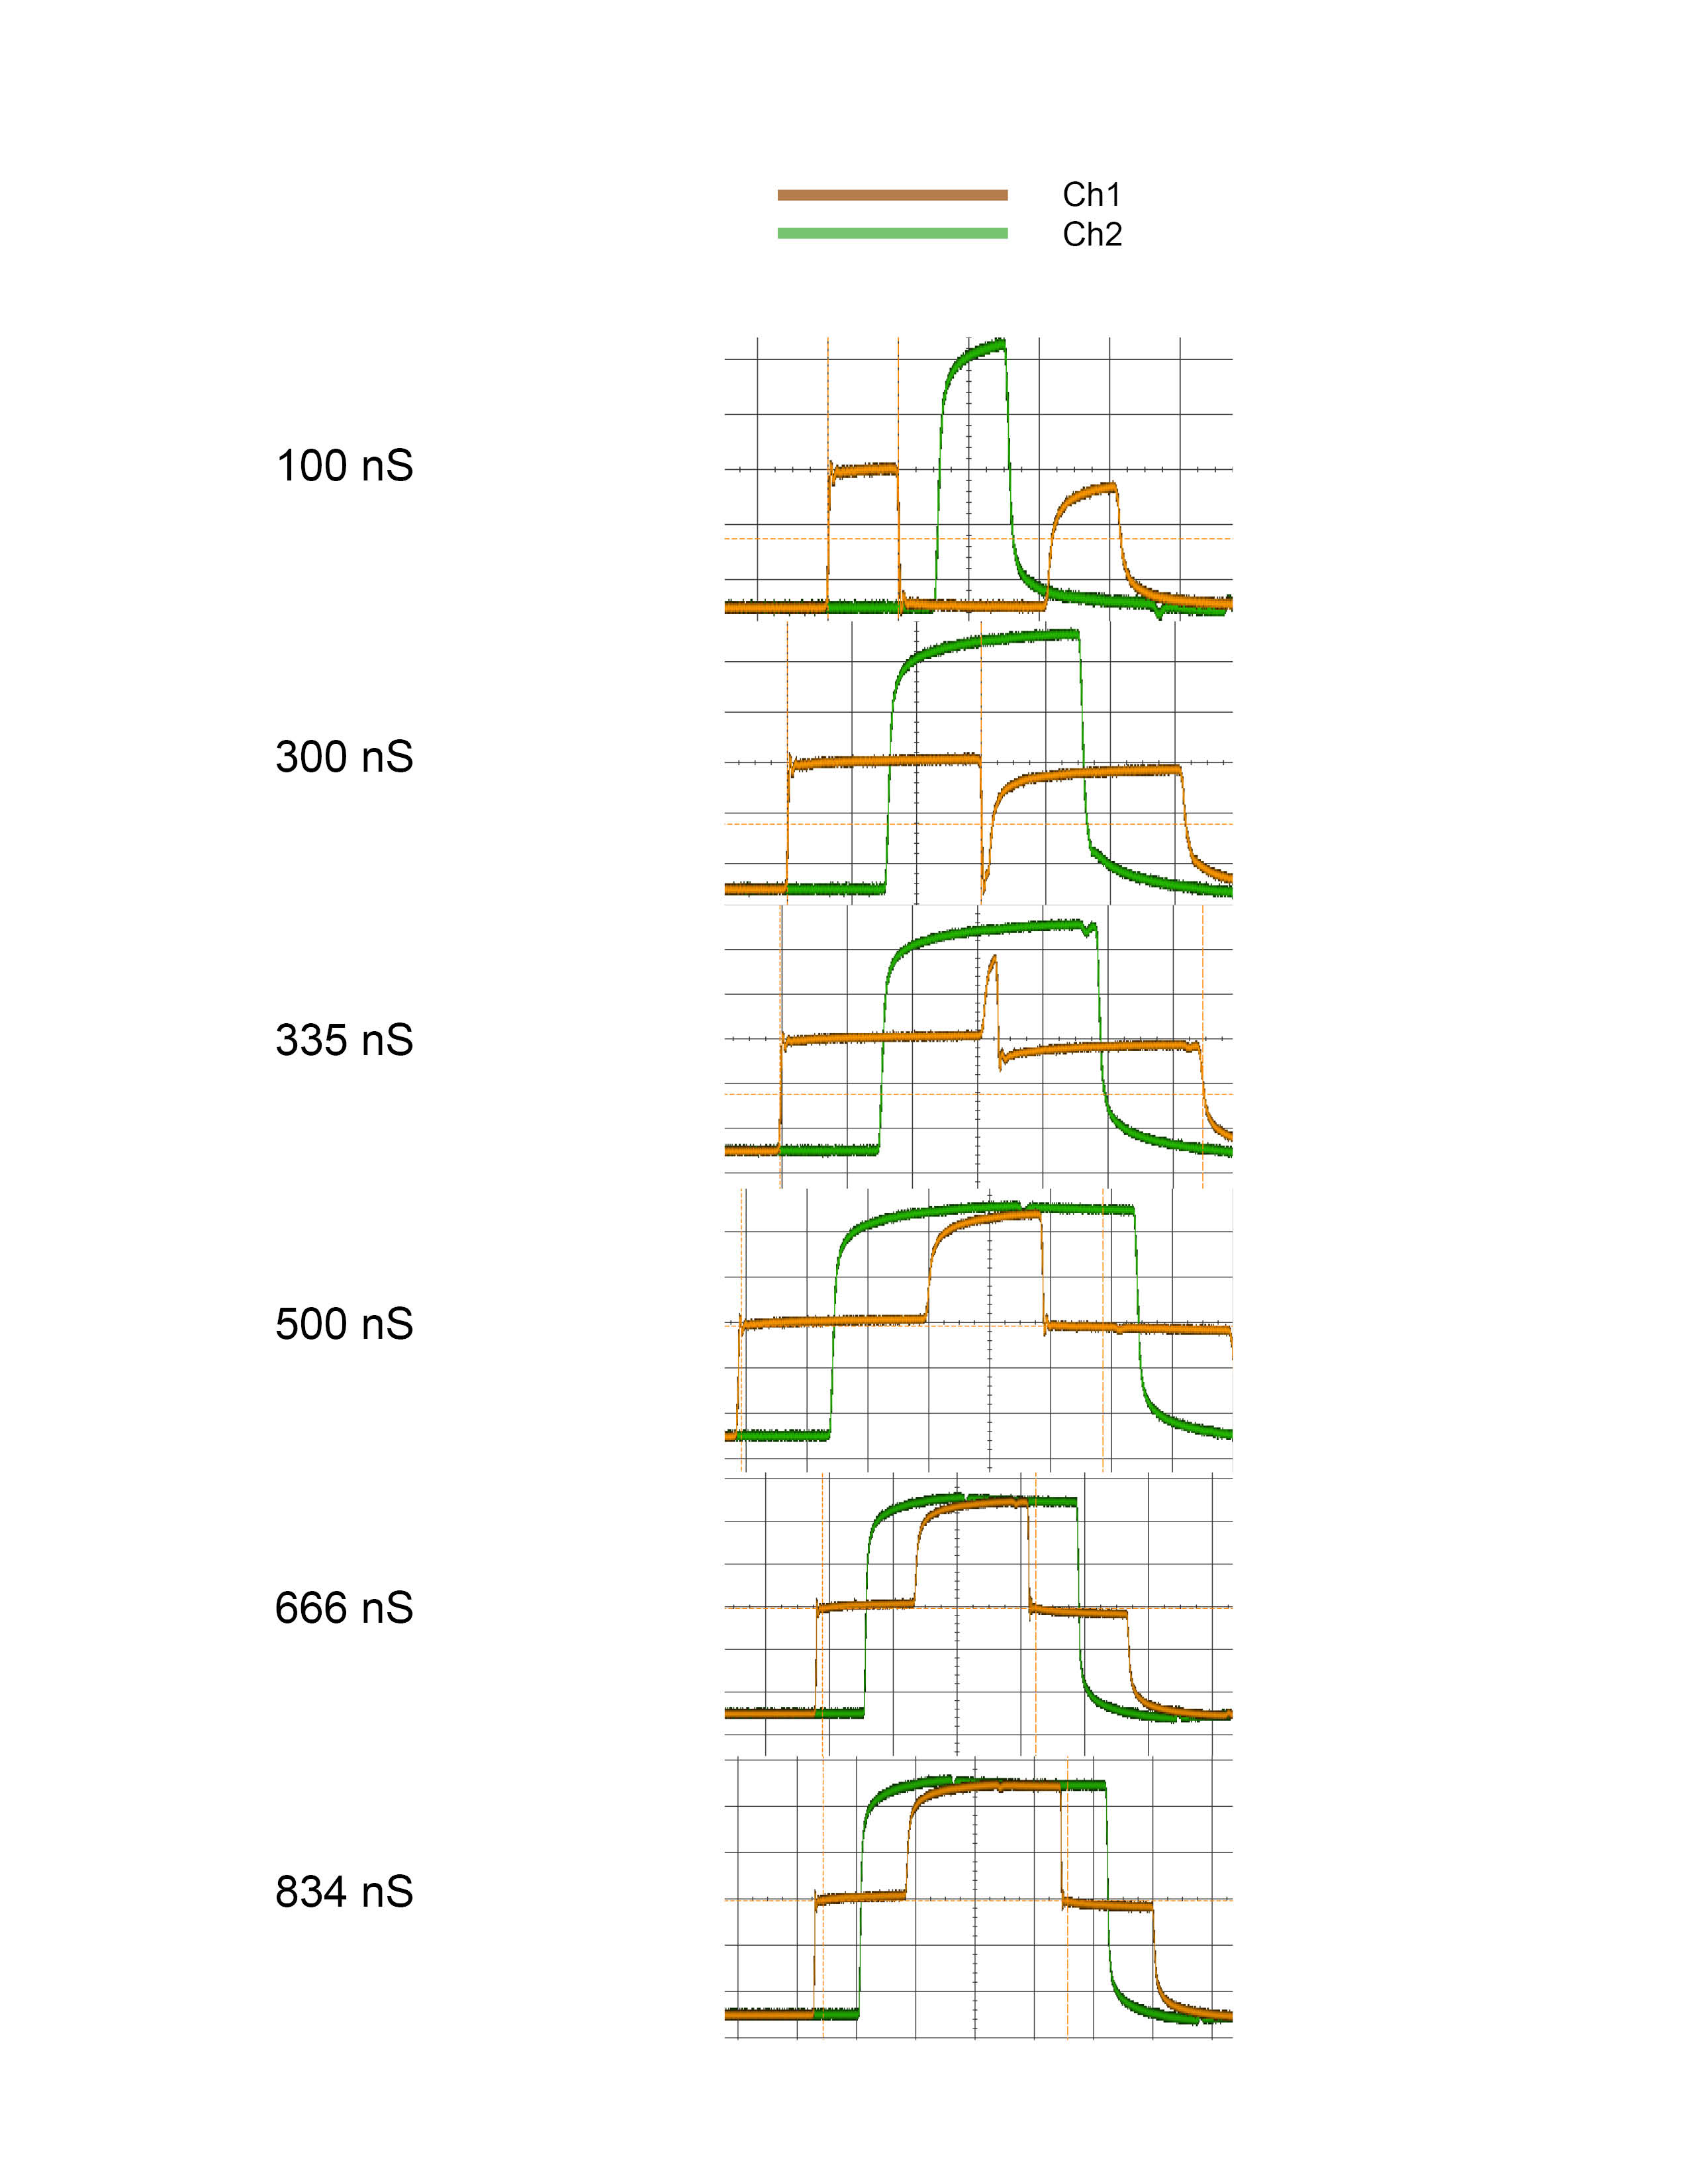
\includegraphics[width=0.7\linewidth]{nudes/A1aAlle.jpg}
    \caption{Spannungsverläufe der jeweiligen Pulsdauern}
    \label{fig:Spannungspulse}
\end{figure}

\noindent
Zu Beginn bei einer Pulsweite von 100 nS lässt sich erkennen, dass der Spannungspuls am Kabelende auftrifft und dort reflektiert wird. 
Bei einem offenem Leiterende liegt der Reflexionskoeffizient bei 1, weshalb es hier zu einer Spannungsverdopplung kommt.
Nach kurzer Zeit kommt der reflektierte Teil auch wieder am Eingang, also dem Kanal 1, an und wird dort detektiert. \newline

\noindent
Bei etwa 335 nS sieht man am Graphen einen Umschwung zwischen der einlaufenden- und der reflektierten Welle.
Hier befindet sich die Grenze, bei der der Puls selbst länger ist, als die Zeit die er hin und zurück benötigt, weshalb sich das Signal hier überlagert.
Diese Überlagerung wird mit zunehmender Pulsdauer weiter vergrößert. \newline

\noindent
In den ermittelten Abbildungen \ref{fig:GraphenB1} und \ref{fig:GraphenB2} wurde nun der Innenwiderstand der Signalquelle erhöht bzw. verringert. \newline

\noindent
Bei erhöhtem Innenwiderstand wird das Signal nun nicht nurnoch am Kabelende, sondern auch am eingebundenen Widerstand reflektiert. 
Dies führt zu einer Addition dieser Widerstände, wodurch die Kabelimpedanz überschritten wird und so ein offenes Kabelende bilden (positive Reflexionsstelle).
Wie in Abbildung \ref{fig:GraphenB1} zu erkennen, wird das eingehende Signal, sobald es am offenen Ende ankommt, reflektiert.
Dies geschiet jedoch erneut, sobald es am Eingang wieder ankommt, was zu einer dreifachen Überlagerung des Signals führt.
Durch die Kabelimpedanz und den nicht unendlichen Abschlusswiderstand wiederholt sich dieser Prozess zwar nun fortlaufend, jedoch wird die Spannung jedesmal etwas abgeschwächt. \newline

\noindent
Mit verringertem Innenwiderstand kommt es zu einem sehr ähnlichen Phänomen.
Wie sich in Abbildung \ref{fig:GraphenB2} sehen lässt, kommt es jedoch zu einem unterschiedlichem Resultat.
Dadurch, dass sich am offenen Ende ebenfalls eine positive Reflexion bildet, am Eingang aber eine negative Reflexion auftritt, kommt es zu einem auf- und abschwankendem Signal.



\subsection{Reflexionskoeffizient/Kabelimpedanz}

Mit den ermittelten Spannungen aus Tabelle \ref{tab:A2Spannungen}, eingesetzt in Formel \ref{eq:Reflexionskoeffizient}, lassen sich die Reflexionskoeffizienten bestimmen.

\begin{table}[H]
    \centering
    \caption{Berechnete Reflexionskoeffizienten der jeweiligen Widerstände}
    \label{tab:Reflexionskoeffizienten}
    \begin{tabular}{| l | l | l | l |}
        \hline
        R / $\Omega$  & $\rho$ / 1 & $\Delta \rho$ / 1 \\
        \hline
       0.676 & -0.79 & 0.11 \\
       0.998 & -0.80 & 0.11 \\
         2.2 & -0.85 & 0.11 \\
        16.1 & -0.53 & 0.11 \\
        16.1 & -0.53 & 0.11 \\
        18.2 & -0.51 & 0.11 \\
        22.1 & -0.38 & 0.10 \\
        33.1 & -0.32 & 0.10 \\
        47.2 & -0.13 & 0.08 \\
        68.6 &  0.17 & 0.07 \\
       100.2 &  0.32 & 0.06 \\
         179 &  0.51 & 0.06 \\
         330 &  0.67 & 0.05 \\
        \hline
    \end{tabular}
\end{table}

\noindent
Mit den resultierenden Werten lässt sich ein Graph zeichnen, welcher den Reflexionskoeffizienten der einzelnen Abschlusswiderstäne aufzeigt (theoretischer Verlauf laut Gleichung \ref{eq:Reflexionskoeffizient} in grün).

\begin{figure}[H]
    \centering
    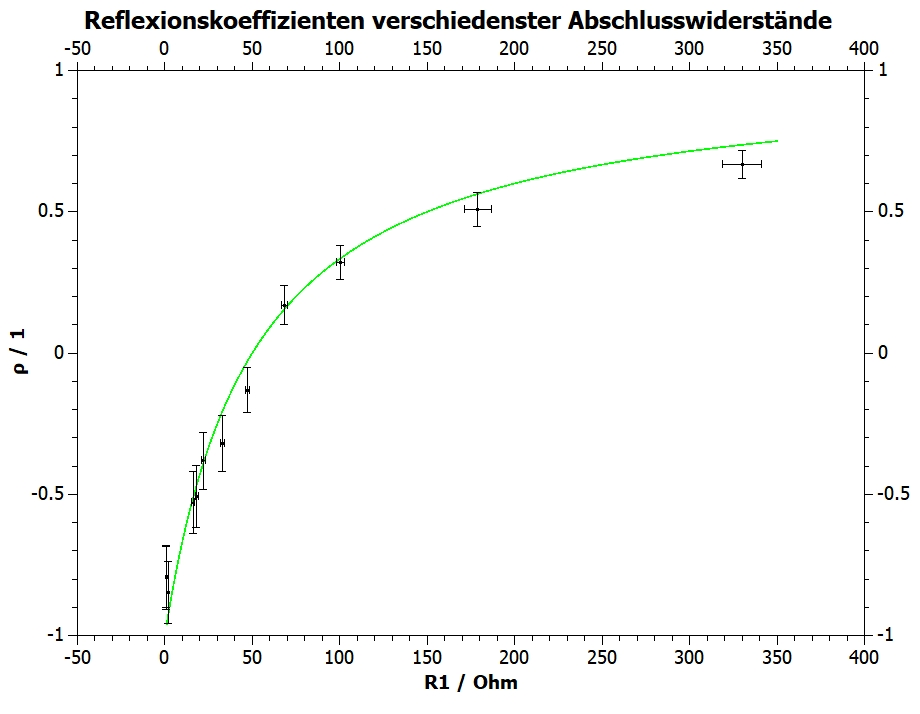
\includegraphics[width=0.7\linewidth]{nudes/Reflexionskoeffizienten Graph.jpg}
    \caption{Reflexionskoeffizienten der verschiedenen Abschlusswiderstände}
    \label{fig:ReflexionskoeffizientenGraph}
\end{figure}

\noindent
Durch lineare Interpolation der Messwerte ergibt sich weiters bei $\rho$ = 0 die Abschlussimpedanz, und laut Gleichung \ref{eq:Reflexionskoeffizient} gleich die Kabelimpedanz von (56.5 $\pm$ 1.6) $\Omega$. \newline

\noindent
Mit den gemessenen Werten aus Tabelle \ref{tab:A2SpannungenBNC} kann mittels Gleichung \ref{eq:Reflexionskoeffizient} der reale Reflexionskoeffizient mit (0.15 $\pm$ 0.09) berechnet werden.


\subsection{Signalgeschwindigkeit/relative Permittivität}

Mit Hilfe der Daten aus Aufgabe 1 (100 nS Puls Messung) kann die Laufzeit t = (300 $\pm$ 10) nS und die Kabellänge s = (31.1 $\pm$ 0.1) m bestimmt werden.
Mittels Formel \ref{eq:Signalgeschwindigkeit} ergibt sich die Signalgeschwindigkeit v. \newline

\noindent
v = (207*$10^6$ $\pm$ 8*$10^6$) m/s \newline

\noindent
Weiters lässt sich mittels Gleichung \ref{eq:Permittivität} die relative Permittivität bestimmen.

\noindent
$\epsilon_r$ = (2.09 $\pm$ 0.13) \newline


\subsection{Verzweiger}

Der Spannungsverlauf des Verteilers wurde am Oszilloskop aufgenommen und ist in Abbildung \ref{fig:GraphA4} ersichtlich.


\section{Diskussion} %diskussion der Unsicherheiten und Ergebnisse und evtl. verlgeich mit Literatur ------------------------------

\subsection{Spannungsverläufe}

Die Spannungsverläufe der jeweiligen Pulsdauer entsprechen den theoretischen Erwartungen.

\subsection{Reflexionskoeffizient/Kabelimpedanz}

Prinzipiell befinden sich die gemessenen Reflexionskoeffizienten im Bereich des theoretischen Verlaufes.
Nur bei den höheren Widerstandswerten weichen die Werte leicht von den Erwartungen ab.
Dies macht aber weitesgehend auch Sinn, da Verluste z.B. im Kabel nicht miteinbezogen wurden.
Die bestimmte Kabelimpedanz von (56.5 $\pm$ 1.6) $\Omega$ kommt dem Literaturwert von 50 $\Omega$ jedoch sehr nahe, wobei auch hier Verluste eine Rolle spielen.


\subsection{Signalgeschwindigkeit/relative Permittivität}

Die Signalgeschwindigkeit, welche im dritten Aufgabenteil bestimmt wurde, liegt zum einen unter der Lichtgeschwindigkeit und im Bereich der 66$\%$ der Lichtgeschwindigkeit (wie bei BNC-Tools üblich), was beides für eine korrekte Durchführung spricht.
Weiters liegt auch die Permittivität mit (2.09 $\pm$ 0.13), verglichen mit anderen Kunstoffen (z.B. Vinyl: 2.2) in einem realistischen Umfeld.


\subsection{Verzweiger}

Die experimentell bestimmten Widerstände ergeben gemeinsam einen Impedanzwert von etwa 50 $\Omega$ und liegen somit ebenfalls in einem denkbaren Bereich.


\section{Zusammenfassung} %klare, übersichtliche vollständige beantwortung der Aufgabenstellung ------------------------------

\subsection{Spannungsverläufe}

Die Spannungsverläufe sind in Abbildung \ref{fig:Spannungspulse} zu erkennen und wurden im Kapitel Auswertung beschrieben.


\subsection{Reflexionskoeffizient/Kabelimpedanz}

\begin{table}[H]
    \centering
    \caption{Berechnete Reflexionskoeffizienten der jeweiligen Widerstände}
    \label{tab:ReflexionskoeffizientenZF}
    \begin{tabular}{| l | l | l | l |}
        \hline
        R / $\Omega$  & $\rho$ / 1 & $\Delta \rho$ / 1 \\
        \hline
       0.676 & -0.79 & 0.11 \\
       0.998 & -0.80 & 0.11 \\
         2.2 & -0.85 & 0.11 \\
        16.1 & -0.53 & 0.11 \\
        16.1 & -0.53 & 0.11 \\
        18.2 & -0.51 & 0.11 \\
        22.1 & -0.38 & 0.10 \\
        33.1 & -0.32 & 0.10 \\
        47.2 & -0.13 & 0.08 \\
        68.6 &  0.17 & 0.07 \\
       100.2 &  0.32 & 0.06 \\
         179 &  0.51 & 0.06 \\
         330 &  0.67 & 0.05 \\
        \hline
    \end{tabular}
\end{table}

\noindent
Der dazugehörige Graph ist mitsamt theoretischem Verlauf in Abbildung \ref{fig:ReflexionskoeffizientenGraph} ersichtlich.
Die berechnete Kabelimpedanz und der gemessene Reflexionskoeffizient betragen (56.5 $\pm$ 1.6) $\Omega$ und (0.15 $\pm$ 0.09).


\subsection{Signalgeschwindigkeit/relative Permittivität}

Die Signalgeschwindigkeit wurde mit v = (207*$10^6$ $\pm$ 8*$10^6$) m/s bestimmt, die Permittivität mit $\epsilon_r$ = (2.09 $\pm$ 0.13).


\subsection{Verzweiger}

Der Verzweiger wurde praktisch realisiert und ein Oszilloskopbild in Abbildung \ref{fig:GraphA4} gespeichert.

\printbibliography[heading=bibintoc]
\end{document}
